\chapter{Análise de Resultados} \label{ch:resultados}
\setlength{\headheight}{13.6pt}
%%%%%%%%%%%%%%%%%%%%%%%%%%%%%%%%%%%%%%%%%%%%%%%%%%%%%
Como referido no Capítulo \ref{ch:intro}, este capítulo é dedicado à exposição e análise dos resultados obtidos das simulações e experimentos realizados ao longo do projeto da ferramenta porta-peças desenvolvida.
\par
Uma vez que os resultados para as tres séries de rodas de coroa são similares, serão discutidos apenas resultados de uma série de rodas de coroa, para isto, foi selecionada a série DB45. A razão da escolha desta série de rodas de coroa não é outra além da disponibilidade dos resultados, uma vez que foi o primeiro ensaio a ser realizado, os resultados estavam disponíveis para serem tratados atempadamente. Pouco antes do final da redação deste documento, também estavam disponíveis os resultados das rodas de coroa de série JT4, e os resultados das rodas de coroa de série DB35 só estariam disponíveis após a data de entrega deste documento.
Para os resultados das simulações, foram necessários calcular as temperaturas de austenitização A\textsubscript{C1} e A\textsubscript{C3} do material, de acordo com as Equações \ref{eq:A_C1} e \ref{eq:A_C3}, respetivamente. A Tabela \ref{tab:temp_sim} indica estes valores, e outros valores importantes para a análise dos resultados das simulações que serão mostradas a seguir, na Secção \ref{sec:resultados_simulacoes}.
%%%%%%%%%%%%%%%%%%%%%%%%%%%%%%%%%%%%%%%%%%%%%%%%%%%%%%%%%%%%%%%%%%%%%%%%%%%%%
\begin{table}[htb]
    \centering
    \caption[Valores de temperatura importantes para a análise de resultados]%
    {Valores de temperaturas críticas, para o Aço 27MC5, antes e após a carbonitruração, respetivamente, importantes para a análise de resultados.}
    \label{tab:temp_sim}
    \begin{tabular}{lrr} 
    \toprule
    \textbf{Ponto Crítico}                  & \multicolumn{1}{c}{\textbf{Temperatura\textsubscript{Base}}} & \multicolumn{1}{c}{\textbf{Temperatura\textsubscript{(Carb.)}}}  \\ 
    \hline\hline
    Início de Austenitização \textbf{(A\textsubscript{C1})} & 707 °C                                            & 707 °C                                               \\
    Final de Austenitização \textbf{(A\textsubscript{C3})}  & 788 °C                                            & 715 °C                                               \\
    Início de Martensite \textbf{(M\textsubscript{S})}      & 370 °C                                            & 188 °C                                               \\
    Final de Martensite \textbf{(M\textsubscript{F})}       & 175 °C                                            & -30 °C                                               \\
    \hline
    Início de Têmpera \textbf{(T\textsubscript{0})}         & \multicolumn{2}{c}{870 °C}                                                                                \\
    Final de Têmpera \textbf{(T\textsubscript{F})}          & \multicolumn{2}{c}{170 °C}                                                                                \\
    \bottomrule
    \end{tabular}
    \end{table}
%%%%%%%%%%%%%%%%%%%%%%%%%%%%%%%%%%%%%%%%%%%%%%%%%%%%%%%%%%%%%%%%%%%%%%%%%%%%%
\newpage
\section{Resultados das simulações} \label{sec:resultados_simulacoes}
Alguns resultados das simulações já foram expostas no Capítulo \ref{ch:materiais} para efeitos de continuidade do documento, no entanto, alguns resultados necessitam ser analisados de forma a perceber as informações que podem ser adquiridas por simulação numérica.
\par
Como foi referido no passado capítulo, foi realizada uma simulação CFD de todos os protótipos desenvolvidos, entretanto, para além do esquema de velocidades do fluido de têmpera, é possível obter outros parâmetros de uma simulação CFD, entre estes, por exemplo, é possível obter os coeficientes de transferência de calor por convecção na interface entre os elementos finitos das rodas de coroa e os elementos finitos do fluido de têmpera, estes valores podem então ser inseridos numa simulação transiente puramente térmica (Ver Figura \ref{fig:simulacao_termica}) onde é possível obter os valores das velocidades de arrefecimento nos vários pontos. Em especial, foram obtidos os valores da velocidade de arrefecimento num ponto do dentado e num ponto do diâmetro interno.
%%%%%%%%%%%%%%%%%%%%%%%%%%%%%%%%%%%%%%%%%%%%%%%%%%%%%%%%%%%%%%%%%%%%%%%%%%%%%
\begin{figure}[htb]
    \centering
    
\includegraphics[width = 0.6\textwidth]{Figures/Cap4/Falta_Imagem.png}
    \caption[Simulação puramente térmica Solidworks]%
    {Add-in do Solidworks simulation thermal para uma simulação puramente térmica.}
    \label{fig:simulacao_termica}
\end{figure}
%%%%%%%%%%%%%%%%%%%%%%%%%%%%%%%%%%%%%%%%%%%%%%%%%%%%%%%%%%%%%%%%%%%%%%%%%%%%%
\par
Concluída a simulação, foram obtidos os valores do tempo em seis pontos, três para o dentado e três para o diâmetro interno. O primeiro ponto, é obtido quando os elementos atingem o valor de temperatura de austenitização A3, o segundo ponto, quando os elementos atingem a temperatura de austenitização A1, por fim, o terceiro ponto, quando os elementos atingem a temperatura de 170 \textdegree C. As Figuras \ref{fig:Dentado} são referentes aos pontos de temperaturas do dentado, e as Figuras \ref{fig:Diametro}
De forma a facilitar a visualização, nos resultados, as rodas de coroa são vistas pelo plano superior. Foram escolhidas sempre as rodas de coroa Nº 6, ou seja, as rodas do meio da coluna, e as simulações foram feitas num modelo CAD sem o dentado, com o objetivo de diminuir o número de elementos utilizados em cada simulação. A tabela \ref{tab:pontos_sim} indica os valores dos pontos e o tempo em cada um deles, que foram retirados das imagens. Com estes valores é então possível determinar a velocidade de arrefecimento nos pontos em questão e então estimar a microestrutura final no dentado e no diâmetro interno. Para além disso, é possível também prever a dureza final nos dois pontos, tendo em conta a microestrutura, a velocidade de arrefecimento e a composição química do material.
\newpage
%%%%%%%%%%%%%%%%%%%%%%%%%%%%%%%%%%%%%%%%%%%%%%%%%%%%%%%%%%%%%%%%%%%%%%%%%%%%%
\begin{figure}[htb]
    \centering
    \begin{subfigure}{.33\textwidth}\
        \centering
        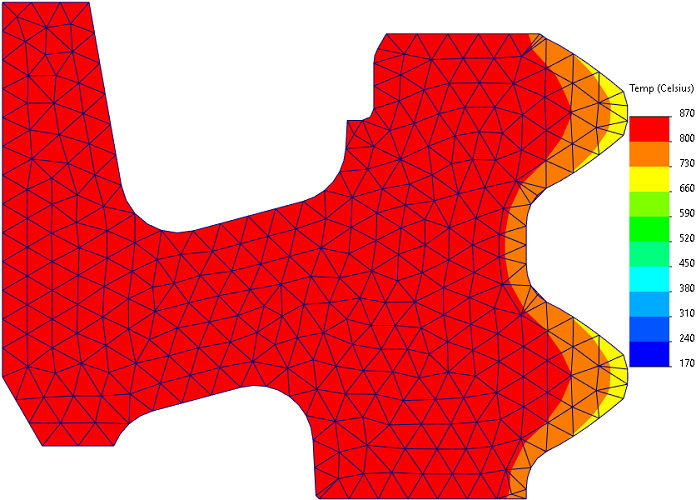
\includegraphics[width = 0.9\textwidth]{Figures/Cap4/Ac3(dentado).png}
        \caption[]%
        {}
        \label{fig:A3_Dent}
    \end{subfigure}%
    \begin{subfigure}{.33\textwidth}
        \centering
        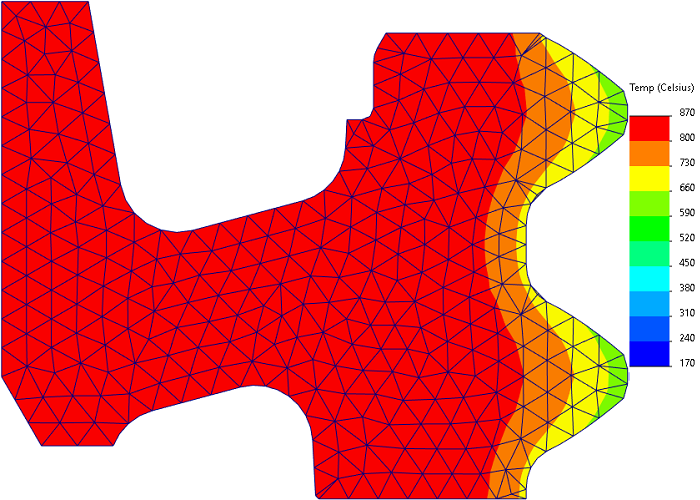
\includegraphics[width = 0.9\textwidth]{Figures/Cap4/Ac1(dentado).png}
        \caption{}
        \label{fig:A1_Dent}
    \end{subfigure}
    \begin{subfigure}{.33\textwidth}
        \centering
        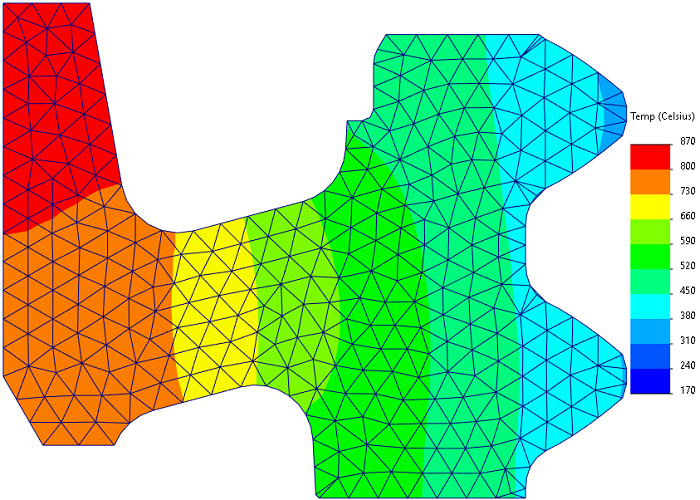
\includegraphics[width = 0.9\textwidth]{Figures/Cap4/Ms(dentado).png}
        \caption{}
        \label{fig:Tf_Dent}
    \end{subfigure}
    \caption[Pontos críticos dos elementos finitos do dentado]%
    {Pontos críticos dos elementos finitos do dentado, para obtenção dos valores de tempo. À esquerda, temperatura A\textsubscript{C1}, que ocorre aos 0,45s, no centro, temperatura A\textsubscript{C3}, que ocorre aos 3,05 s, e à direita, temperatura T\textsubscript{F}, aos 42,00s.}
    \label{fig:Dentado}
\end{figure}
%%%%%%%%%%%%%%%%%%%%%%%%%%%%%%%%%%%%%%%%%%%%%%%%%%%%%%%%%%%%%%%%%%%%%%%%%%%%%
%%%%%%%%%%%%%%%%%%%%%%%%%%%%%%%%%%%%%%%%%%%%%%%%%%%%%%%%%%%%%%%%%%%%%%%%%%%%%
\begin{figure}[htb]
    \centering
    \begin{subfigure}{.33\textwidth}\
        \centering
        
\includegraphics[width = 0.9\textwidth]{Figures/Cap4/Falta_Imagem.png}
        \caption[]%
        {}
        \label{fig:A3_Dint}
    \end{subfigure}%
    \begin{subfigure}{.33\textwidth}
        \centering
        
\includegraphics[width = 0.9\textwidth]{Figures/Cap4/Falta_Imagem.png}
        \caption{}
        \label{fig:A1_Dint}
    \end{subfigure}
    \begin{subfigure}{.33\textwidth}
        \centering
        
\includegraphics[width = 0.9\textwidth]{Figures/Cap4/Falta_Imagem.png}
        \caption{}
        \label{fig:Tf_Dint}
    \end{subfigure}
    \caption[Pontos críticos dos elementos finitos do diâmetro interno]%
    {Pontos críticos dos elementos finitos do diâmetro interno, para obtenção dos valores de tempo. À esquerda, temperatura A\textsubscript{C1}, que ocorre aos 27,65s, no centro, temperatura A\textsubscript{C3}, que ocorre aos 47,15 s, e à direita, temperatura T\textsubscript{F}, aos 270,00s.}
    \label{fig:Diametro}
\end{figure}
%%%%%%%%%%%%%%%%%%%%%%%%%%%%%%%%%%%%%%%%%%%%%%%%%%%%%%%%%%%%%%%%%%%%%%%%%%%%%
\par Nota-se que foi utilizado uma taxa de carbono de 0,7\% no dentado e de 0,24\% no diâmetro interno, o que pode não ser real porque nao se pode garantir que nao haja enriquecimento de carbono no diâmetro interno, mas, uma vez que nao há maneira de prever o valor final da percentagem de carbono no diâmetro interno, optou-se por utilizar o valor do material de base. De acordo com os valores adquiridos, então é possível estimar uma velocidade de arrefecimento média de 35,0\textdegree C/s para o dentado, e uma velocidade de arrefecimento média de 4,7\textdegree C/s para o diâmetro interno.
\par
Para o dentado, estima-se níveis de dureza de cerca de 860HV para uma microestrutura maioritariamente martensítica, e 290HV para uma microestrutura maioritariamente ferrítica e perlítica. Já para o diâmetro interno, considerando que nao haja enriquecimento, estima-se que numa estrutura maioritariamente martensítica, os níveis de dureza estejam por volta de 500HV, e para uma estrutura maioritariamente ferrítica e perlítica, por vota de 190HV.
%%%%%%%%%%%%%%%%%%%%%%%%%%%%%%%%%%%%%%%%%%%%%%%%%%%%%%%%%%%%%%%%%%%%%%%%%%%%%
\begin{table}[htb]
    \centering
    \refstepcounter{table}
    \caption[Valores temporais para cada temperatura crítica]{Valores temporais para cada temperatura crítica no dentado e no diâmetro interno.}
    \label{tab:pontos_sim}
    \begin{tabular}{lr} 
    \toprule
    \multicolumn{1}{c}{\textbf{Ponto Crítico}}            & \multicolumn{1}{c}{\textbf{Tempo (s)}}                         \\ 
    \hline\hline
    Início de Têmpera (T\textsubscript{0})                                & 0,00 s                                         \\ 
    \hline
    Final de Austenitização no dentado (A\textsubscript{C3\_t})           & 0,45 s                                         \\
    Início de Austenitização no dentado (A\textsubscript{C1\_t})          & 3,05 s                                         \\
    Final de Têmpera no dentado (T\textsubscript{F\_t})                   & 42,00 s                                        \\ 
    \hline\hline
    Final de Austenitização no dentado (A\textsubscript{C3\_t})           & 27,65 s                                        \\
    Início de Austenitização no diâmetro interno (A\textsubscript{C1\_d}) & 47,15 s                                        \\ 
    Final de Têmpera (T\textsubscript{F\_d})                              & 270,00 s                                       \\
    \bottomrule
    \end{tabular}
\end{table}
%%%%%%%%%%%%%%%%%%%%%%%%%%%%%%%%%%%%%%%%%%%%%%%%%%%%%%%%%%%%%%%%%%%%%%%%%%%%%
\par
Uma vez que para as velocidades de arrefecimento em questão, o dentado tem em sua maioria martensite e o diâmetro interno, ferrite e perlite. Por consequência, são esperadas durezas por volta de 860HV para o dentado e 190HV para o diâmetro interno. Novamente, deve-se ter em consideração que estas estimativas são para o material que não passa pelo processo de revenido, no caso do dentado, e não sofre enriquecimento de carbono, no caso do diâmetro interno. No caso do material passar por um processo de revenido, o nível de durezas deve reduzir. De igual maneira, no caso de haver enriquecimento de carbono no diâmetro, o nível de durezas deve aumentar.
%%%%%%%%%%%%%%%%%%%%%%%%%%%%%%%%%%%%%%%%%%%%%%%%%%%%%%%%%%%%%%%%%%%%%%%%%%%%%
\section{Resultados do ensaio inicial} \label{sec:resultados_ensaio_inicial}
Como ja foi dito no Capítulo \ref{ch:materiais}, os resultados do protótipo inicial, ou seja, da coluna protegida pela tampa P, foram aquém do esperado. A hipótese que se utiliza para explicar os resultados, é que os três "pingos" de solda feitos para isolar o diâmetro interno das coroas desta coluna partiram, provavelmente por expansão térmica. De qualquer maneira, as Figuras \ref{fig:resultados_Tampa_P_inicial} e \ref{fig:resultados_Serie_inicial} ilustram a diferença entre ter o diâmetro interno tamponado e livre para passagem de fluido de têmpera. De acordo com as Figuras \ref{fig:resultados_Tampa_P_inicial_dent} e \ref{fig:resultados_Serie_inicial_dent}, também é possível ver que o tamponamento do diâmetro interno não tem alterações significativas na filiação de durezas do dentado, confirmando as vantagens da existência de uma ferramenta que protege o diâmetro interno das rodas de coroa.
%%%%%%%%%%%%%%%%%%%%%%%%%%%%%%%%%%%%%%%%%%%%%%%%%%%%%%%%%%%%%%%%%%%%%%%%%%%%%
\begin{figure}[htb]
    \centering
    \begin{subfigure}{.4\textwidth}
        \centering
        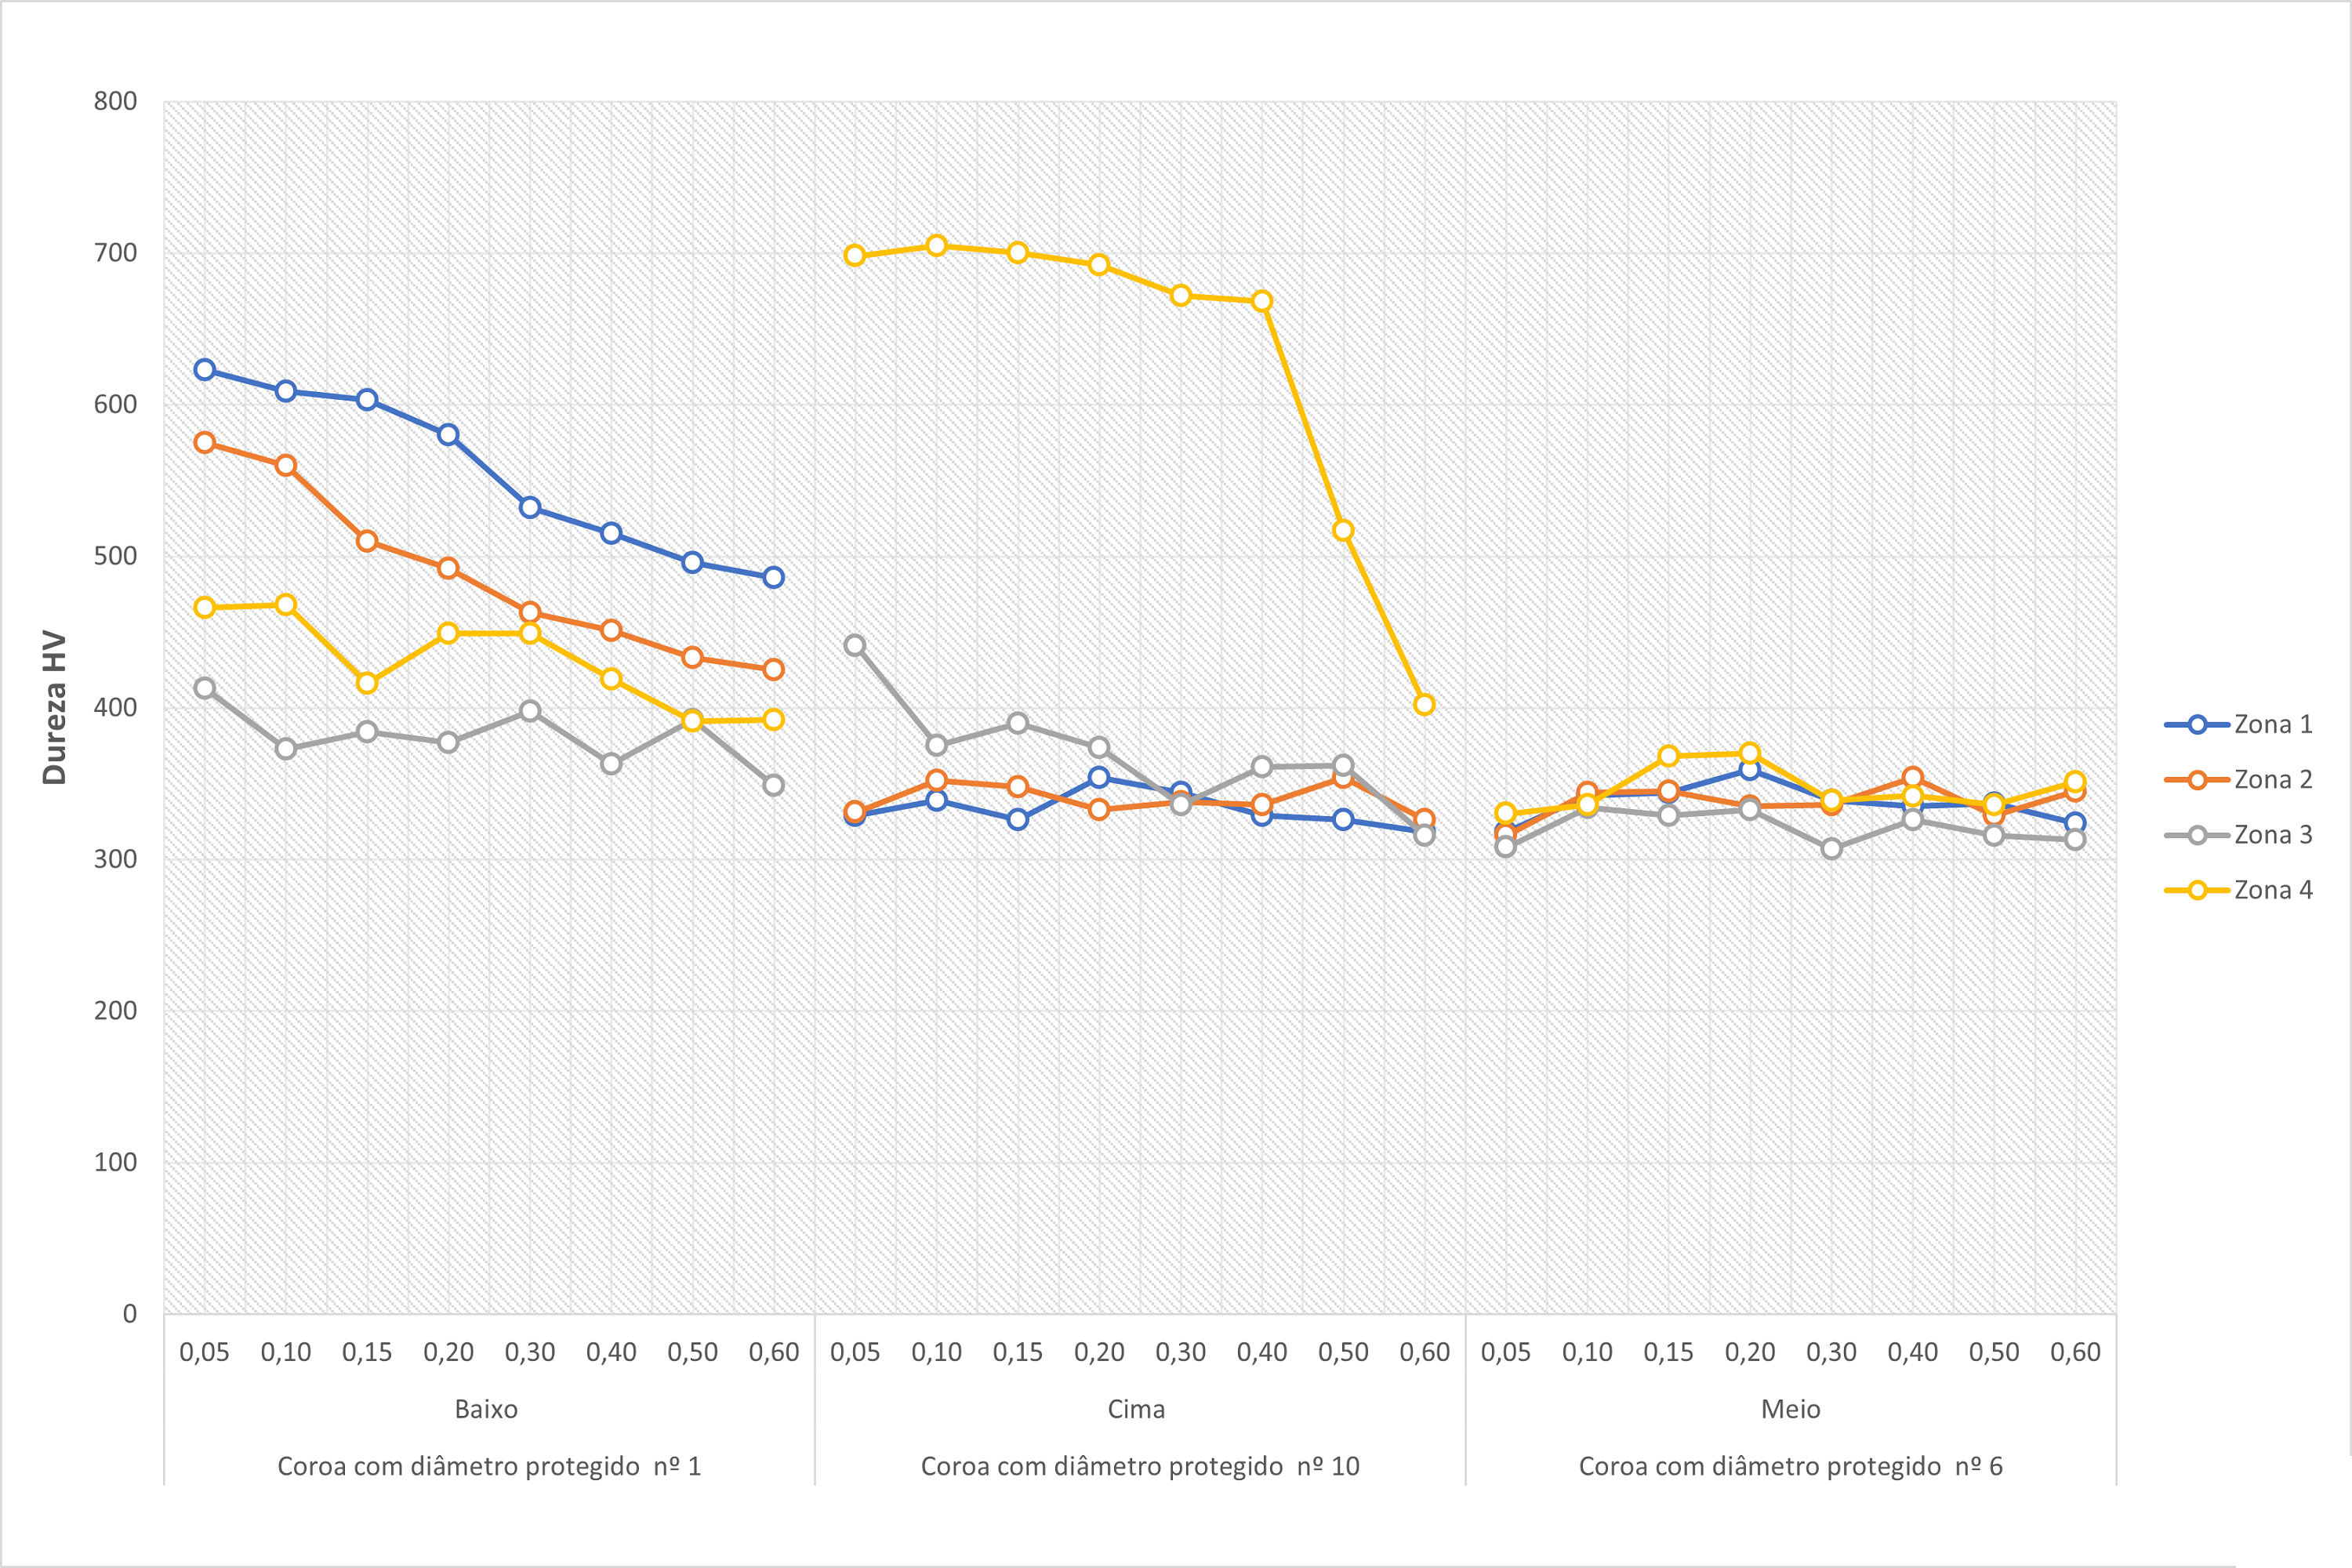
\includegraphics[width = 0.9\textwidth]{Figures/Cap4/Grafico_4_Zonas_P_inicial.png}
        \caption[]%
        {}
        \label{fig:resultados_Tampa_P_inicial}
    \end{subfigure}%
    \begin{subfigure}{.4\textwidth}
        \centering
        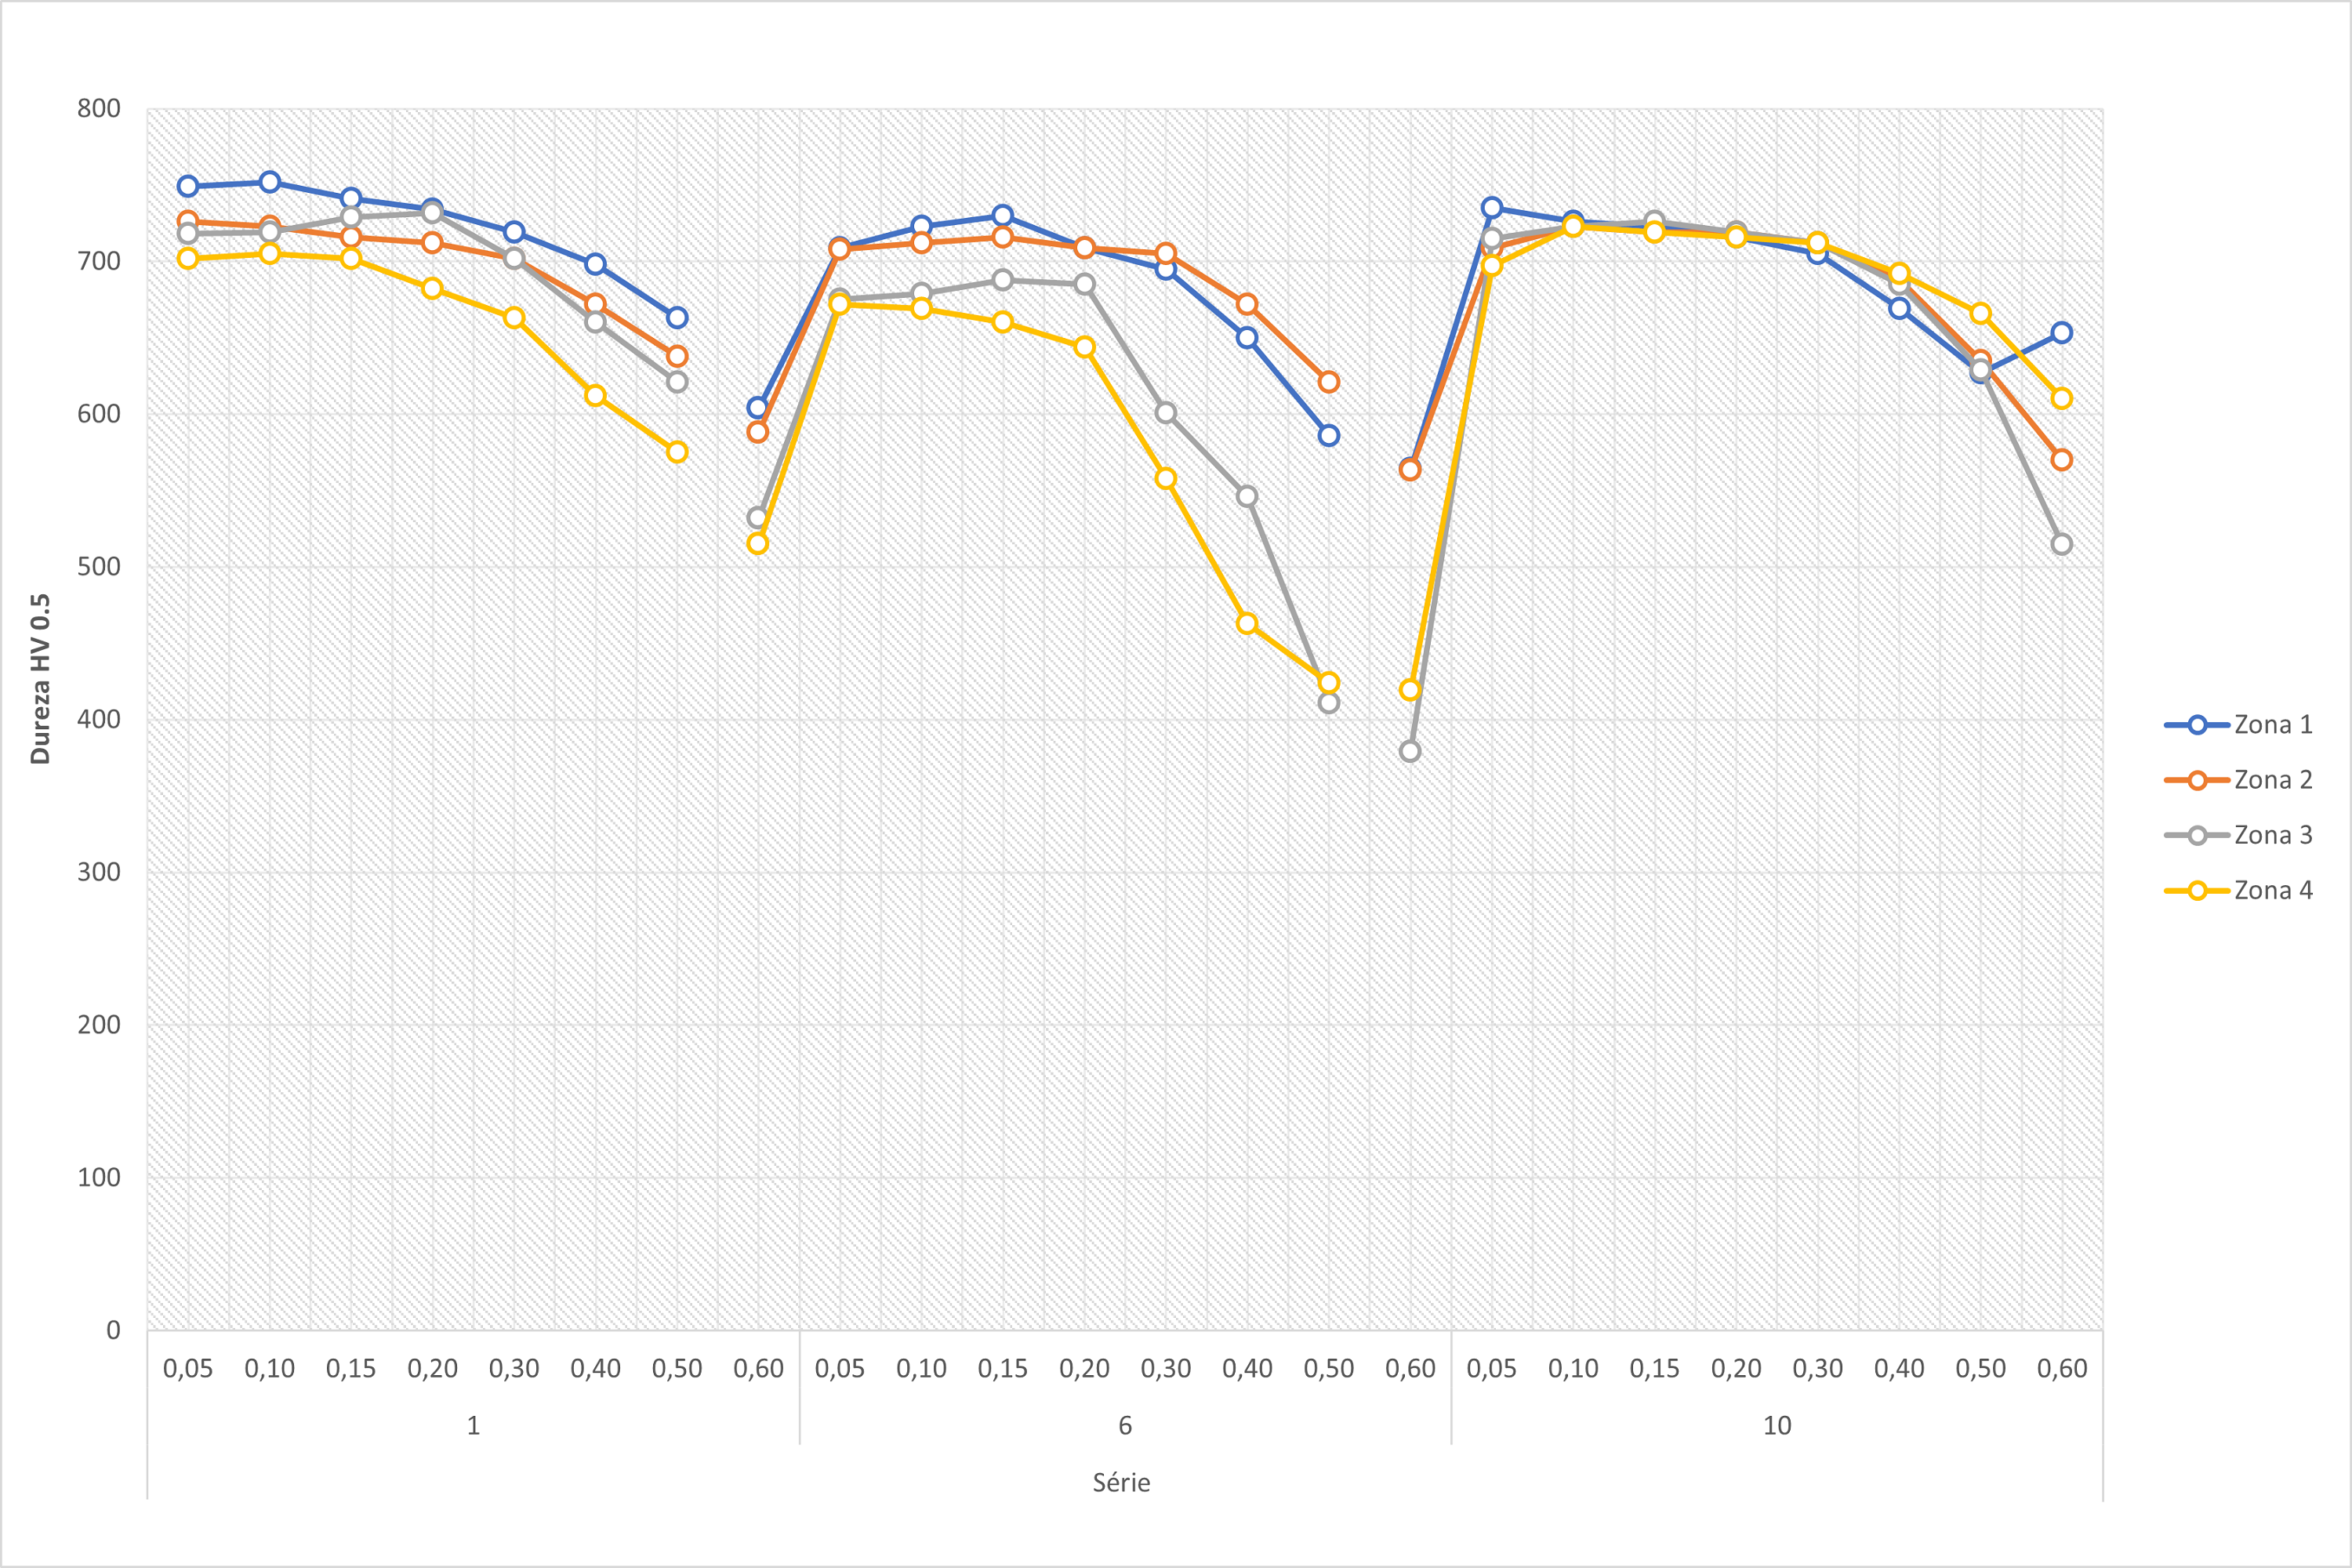
\includegraphics[width = 0.9\textwidth]{Figures/Cap4/Grafico_4_Zonas_S_inicial.png}
        \caption{}
        \label{fig:resultados_Serie_inicial}
    \end{subfigure}
    \begin{subfigure}{.4\textwidth}
        \centering
        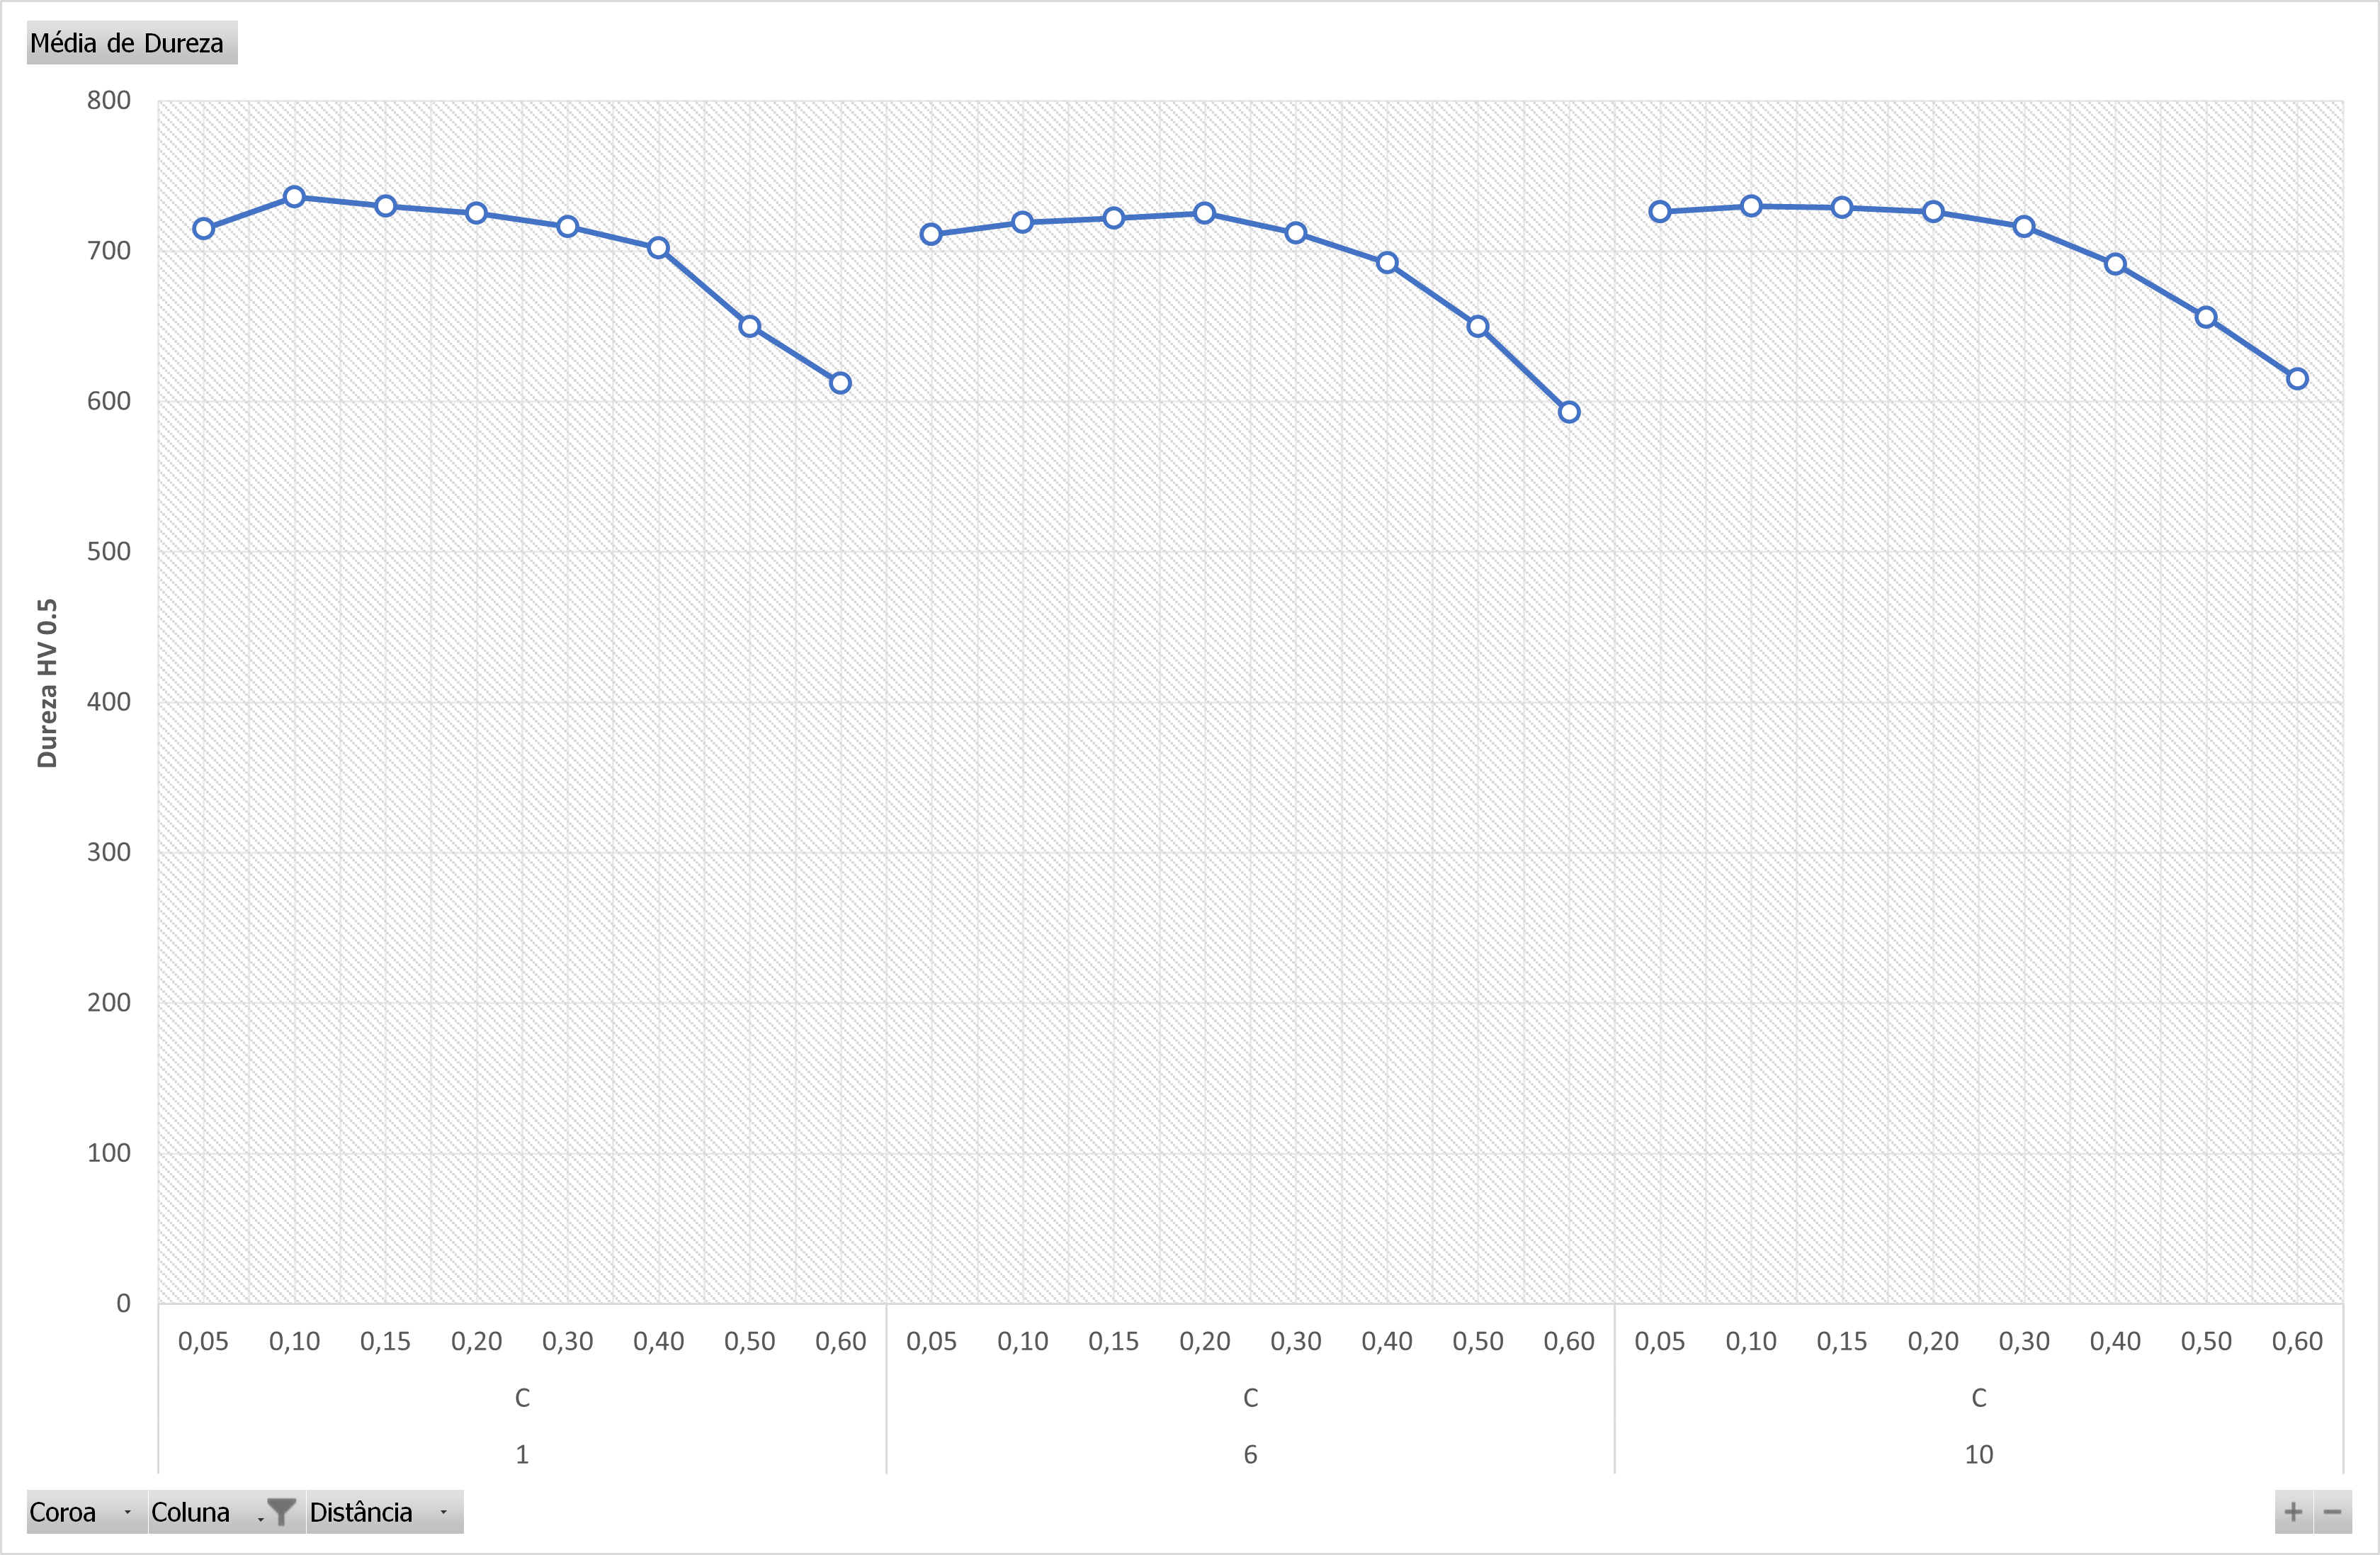
\includegraphics[width = 0.9\textwidth]{Figures/Cap4/Grafico_4_Zonas_P_inicial_dentado.png}
        \caption[]%
        {}
        \label{fig:resultados_Tampa_P_inicial_dent}
    \end{subfigure}%
    \begin{subfigure}{.4\textwidth}
        \centering
        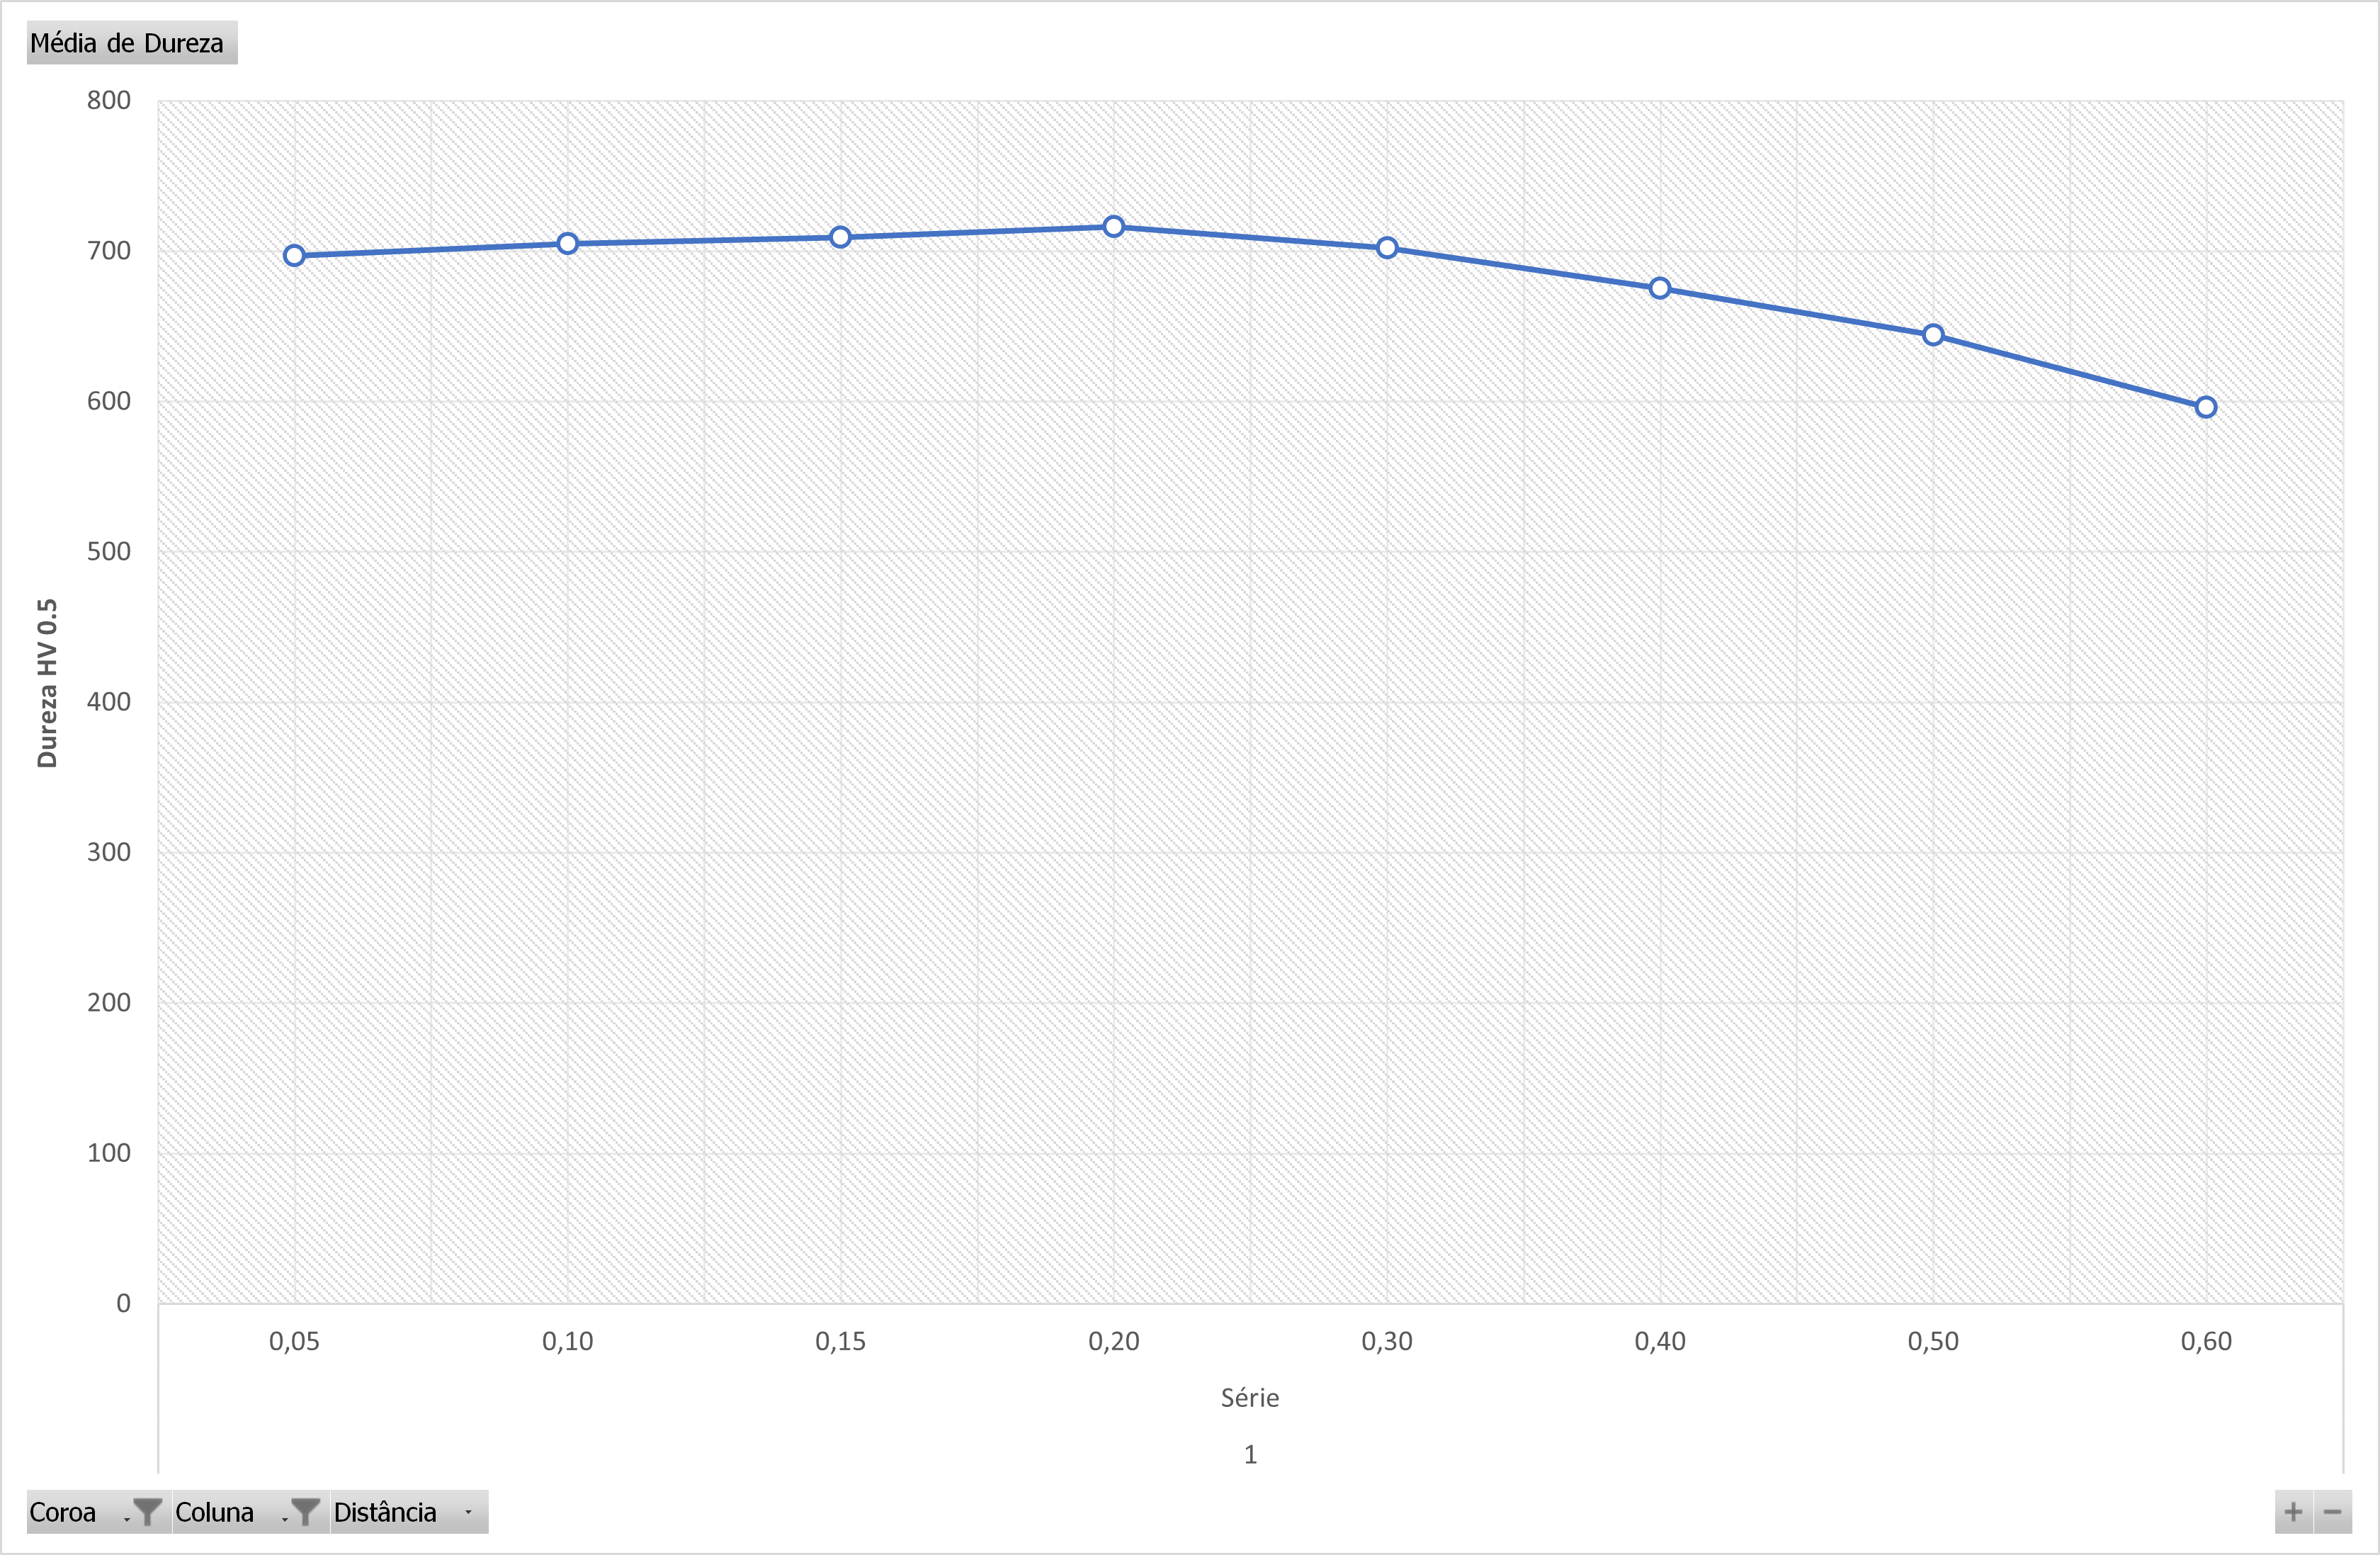
\includegraphics[width = 0.9\textwidth]{Figures/Cap4/Grafico_4_Zonas_S_inicial_dentado.png}
        \caption{}
        \label{fig:resultados_Serie_inicial_dent}
    \end{subfigure}
    \caption[Resultados do ensaio inicial e comparação com peças de série]%
    {Resultados das filiações de dureza obtidas no ensaio inicial, no diâmetro interno e no dentado, e comparação dos valores obtidos nos mesmos pontos nas peças de série.}
\end{figure}
%%%%%%%%%%%%%%%%%%%%%%%%%%%%%%%%%%%%%%%%%%%%%%%%%%%%%%%%%%%%%%%%%%%%%%%%%%%%%
\newpage
\par
É importante perceber que os valores de dureza no diâmetro interno estão muito acima dos valores estimados teoricamente, o que reforça a teoria de que há algum enriquecimento de carbono no diâmetro interno das rodas de coroa protegidas. Outro fator importante de ser mencionado, é que na roda de coroa de cima, na zona 4, há um ganho enorme de dureza. Isso pode ser explicado pela geometria da tampa P, que apenas faz batente na zona 4, portanto, esta zona é apenas protegida a partir de certo ponto, o que também explica a queda brusca na dureza a partir dos 0,40mm de profundidade. Por fim, também é verificado o impacto da rotura da soldadura da falsa coroa na torre da ferramenta porta-peças, sendo assim, é permitida alguma passagem de fluido de têmpera, que causa um aumento significativo nos níveis de dureza da roda de coroa de baixo.
%%%%%%%%%%%%%%%%%%%%%%%%%%%%%%%%%%%%%%%%%%%%%%%%%%%%%%%%%%%%%%%%%%%%%%%%%%%%%
\section{Resultados do ensaio dos protótipos melhorados} \label{sec:resultados_ensaios}
Sendo os resultados da tampa P influenciados pelos "defeitos" mencionados na secção anterior, são expostos os resultados das ferramentas melhoradas, com a adição dos resultados da tampa P após a falsa coroa ser soldada por completo na torre. Novamente, como ponto de comparação dos resultados, visualiza-se os dados das Figuras \ref{fig:resultados_Serie_inicial}, e \ref{fig:resultados_Serie_inicial_dent}.
%%%%%%%%%%%%%%%%%%%%%%%%%%%%%%%%%%%%%%%%%%%%%%%%%%%%%%%%%%%%%%%%%%%%%%%%%%%%%
\begin{figure}[htb]
    \centering
    \begin{subfigure}{.4\textwidth}\
        \centering
        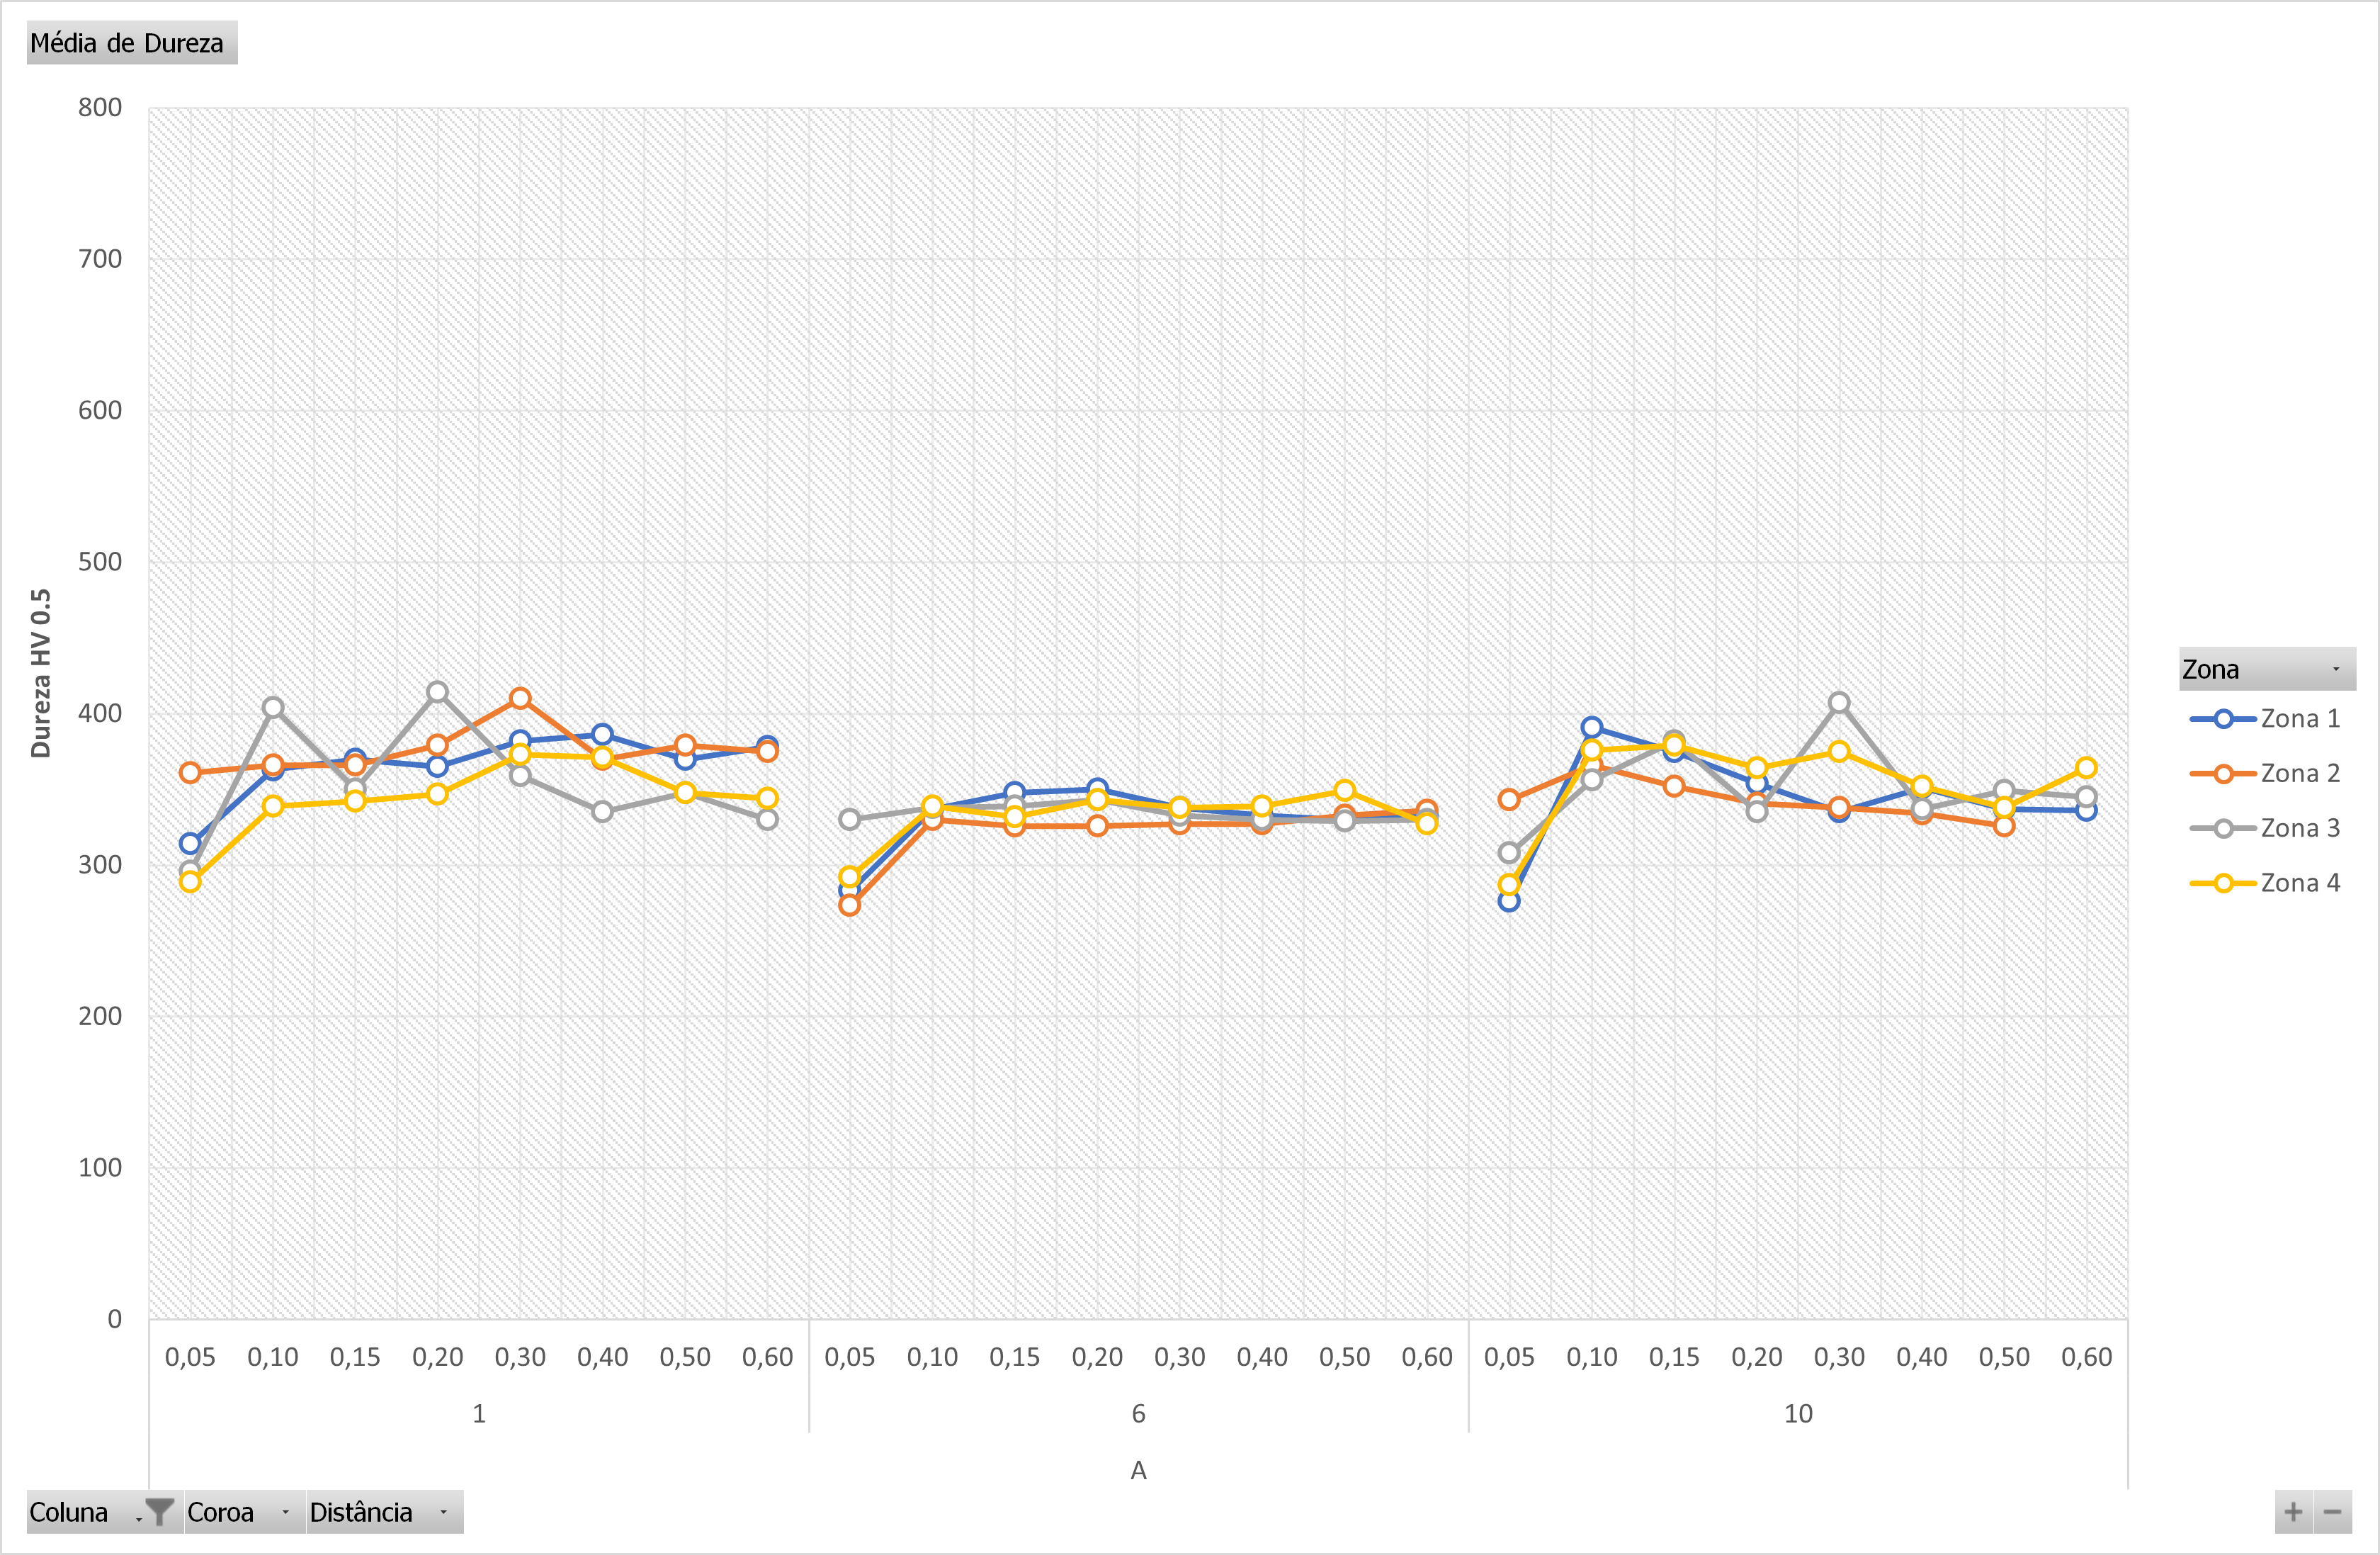
\includegraphics[width = 0.9\textwidth]{Figures/Cap4/Grafico_4_Zonas_Y.png}
        \caption{}
        \label{fig:resultados_Tampa_Y}
    \end{subfigure}%
    \begin{subfigure}{.4\textwidth}
        \centering
        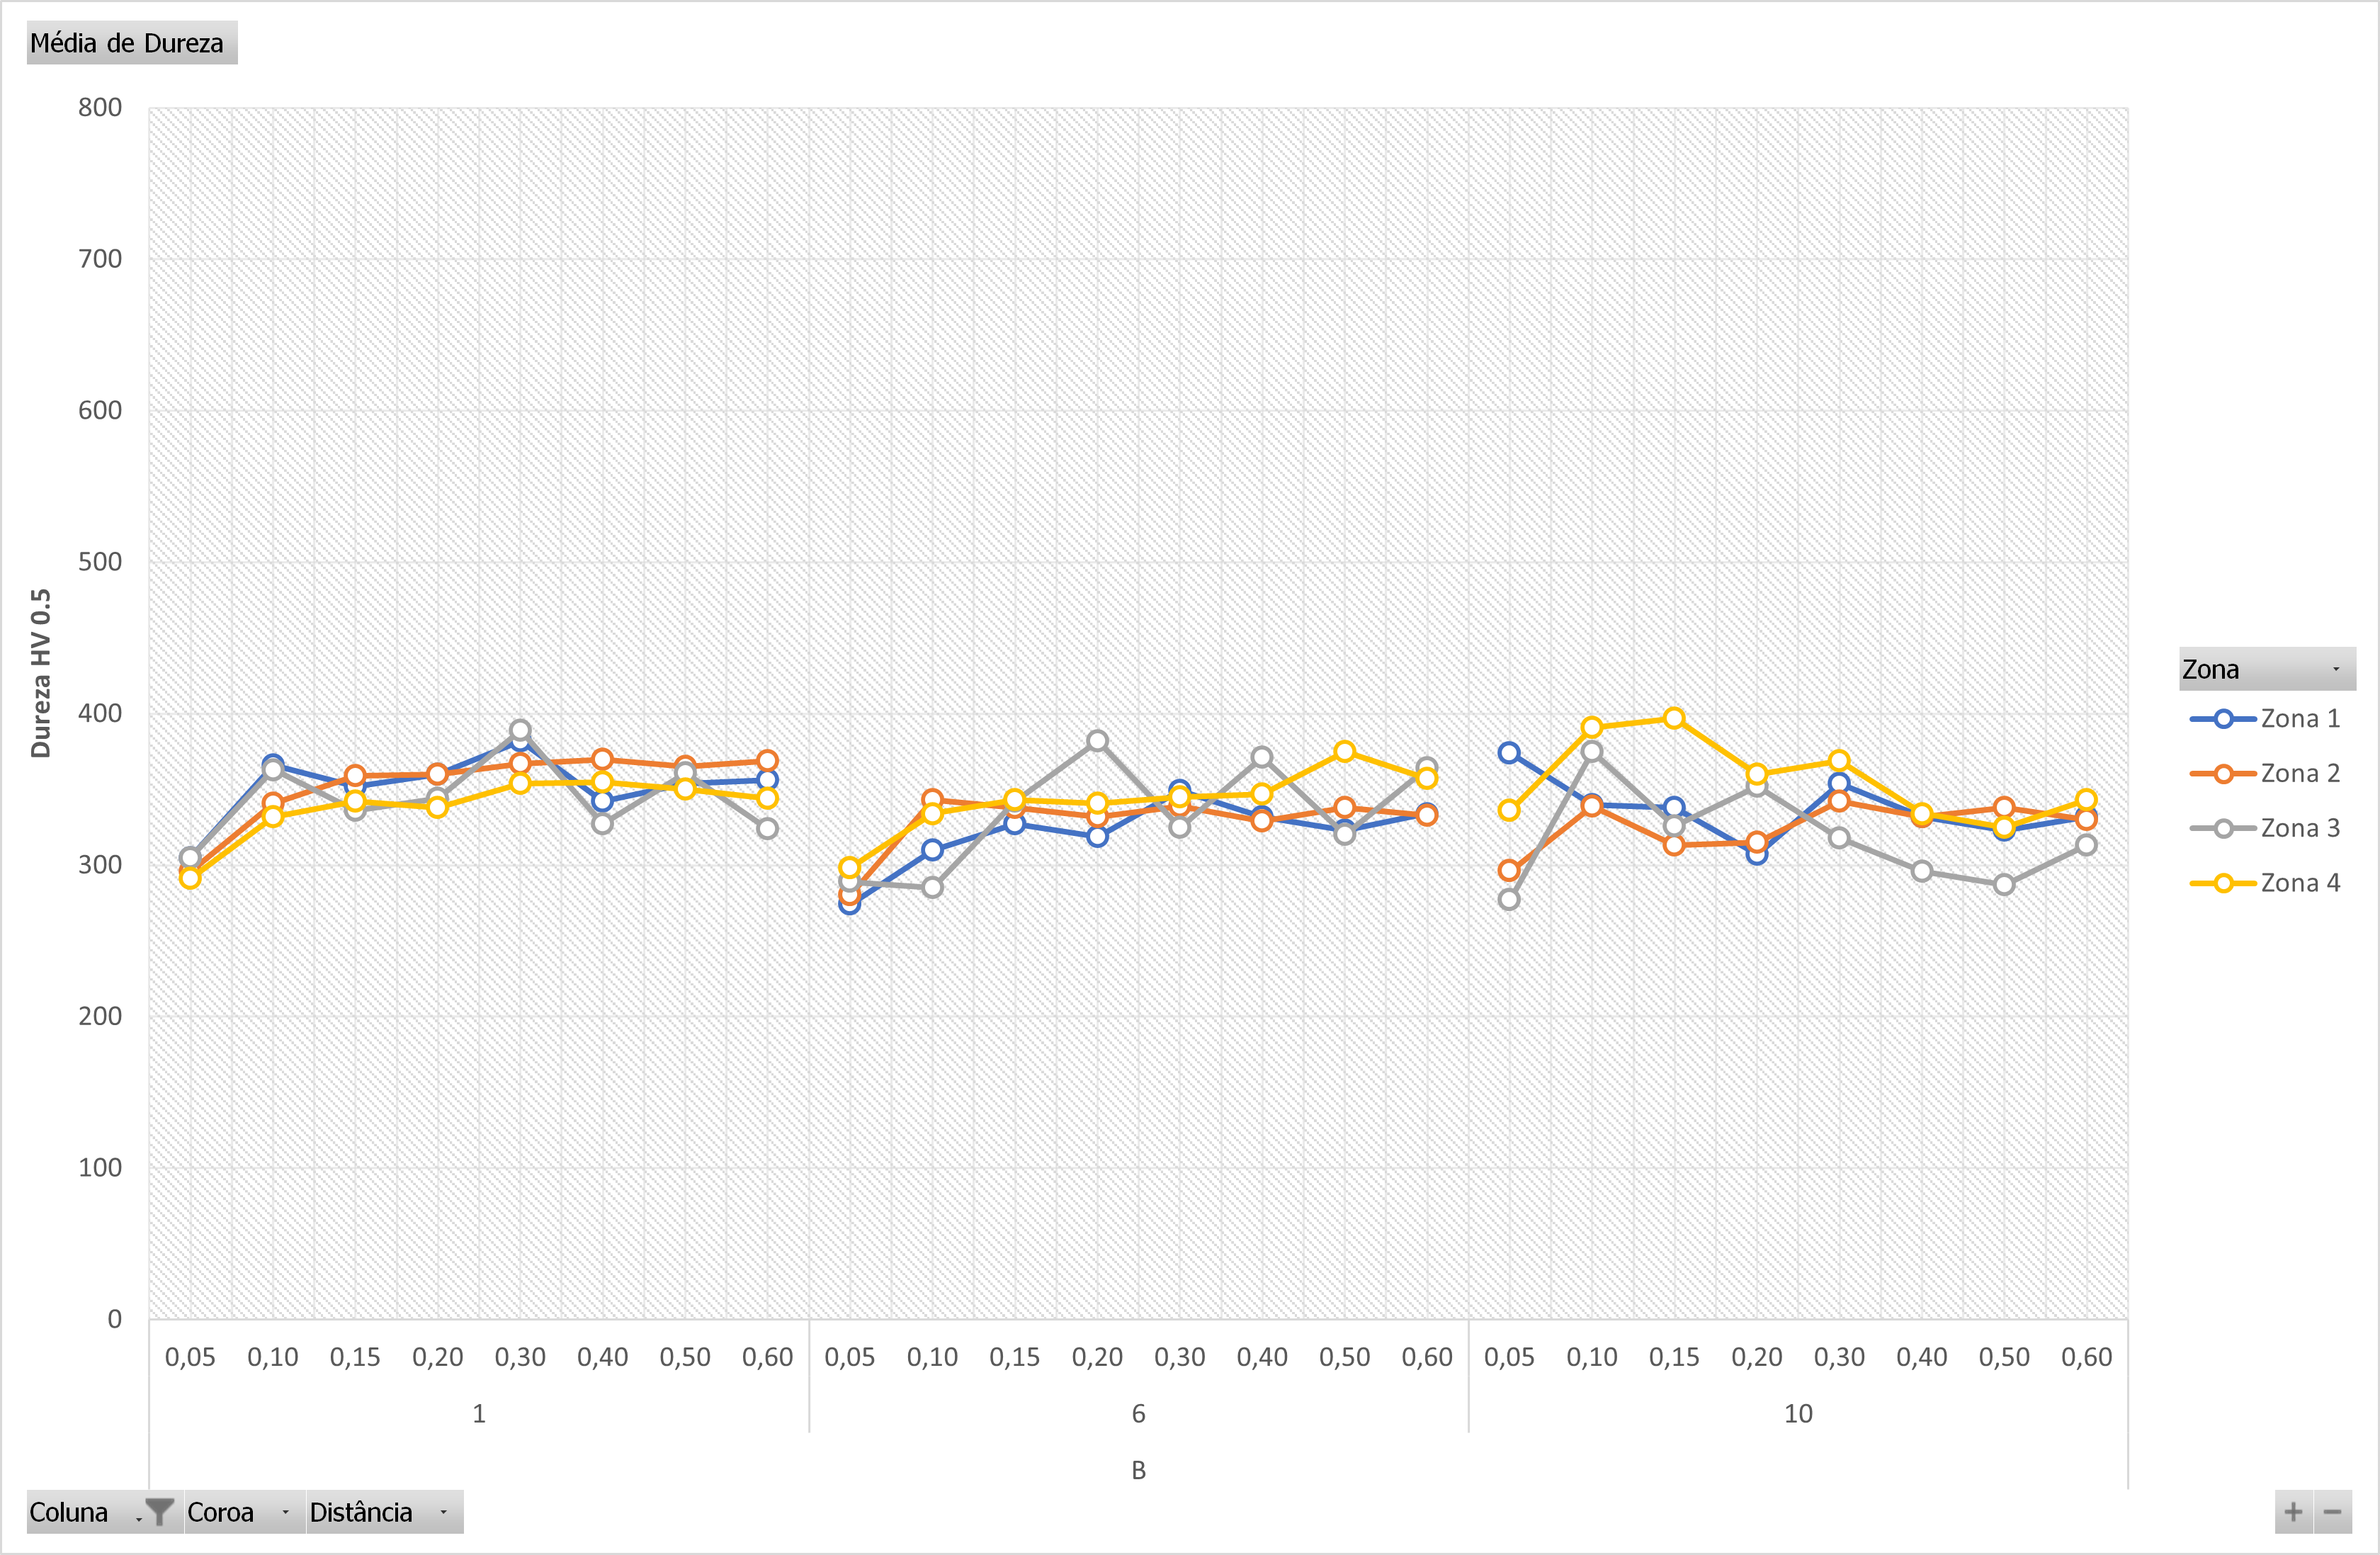
\includegraphics[width = 0.9\textwidth]{Figures/Cap4/Grafico_4_Zonas_O.png}
        \caption{}
        \label{fig:resultados_Tampa_O}
    \end{subfigure}
    \begin{subfigure}{.4\textwidth}\
        \centering
        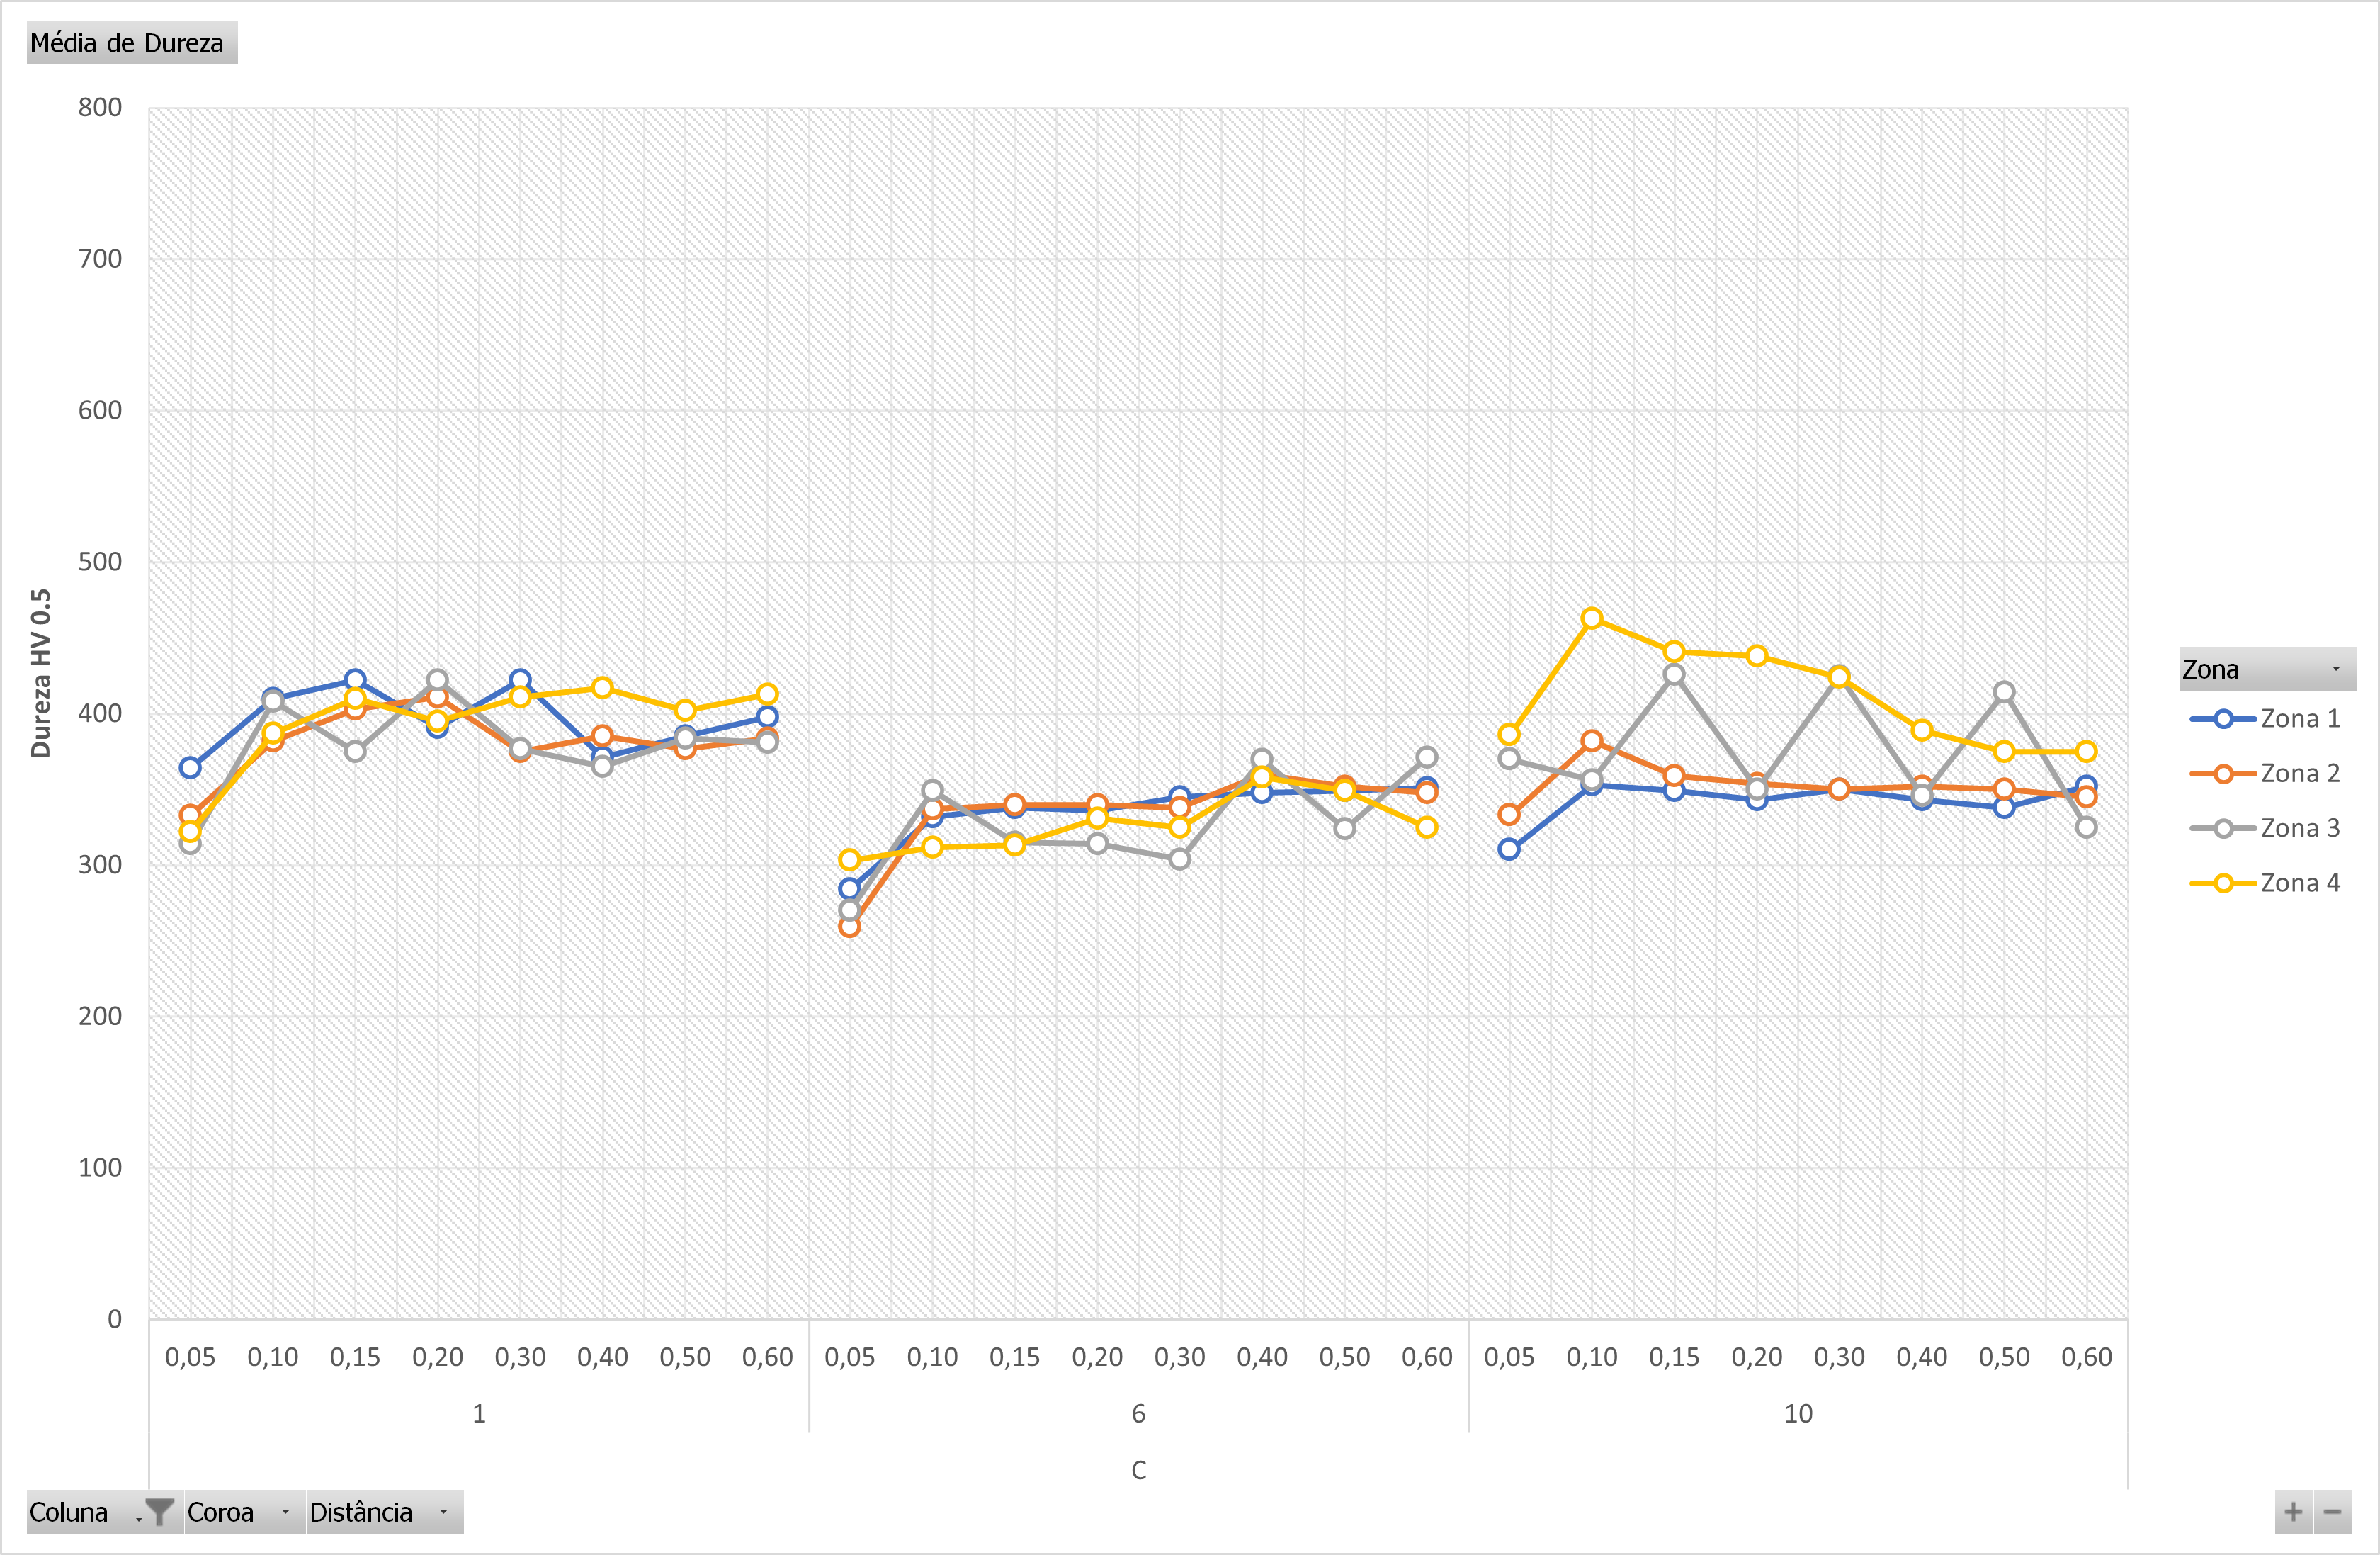
\includegraphics[width = 0.9\textwidth]{Figures/Cap4/Grafico_4_Zonas_P.png}
        \caption{}
        \label{fig:resultados_Tampa_P}
    \end{subfigure}%
    \begin{subfigure}{.4\textwidth}
        \centering
        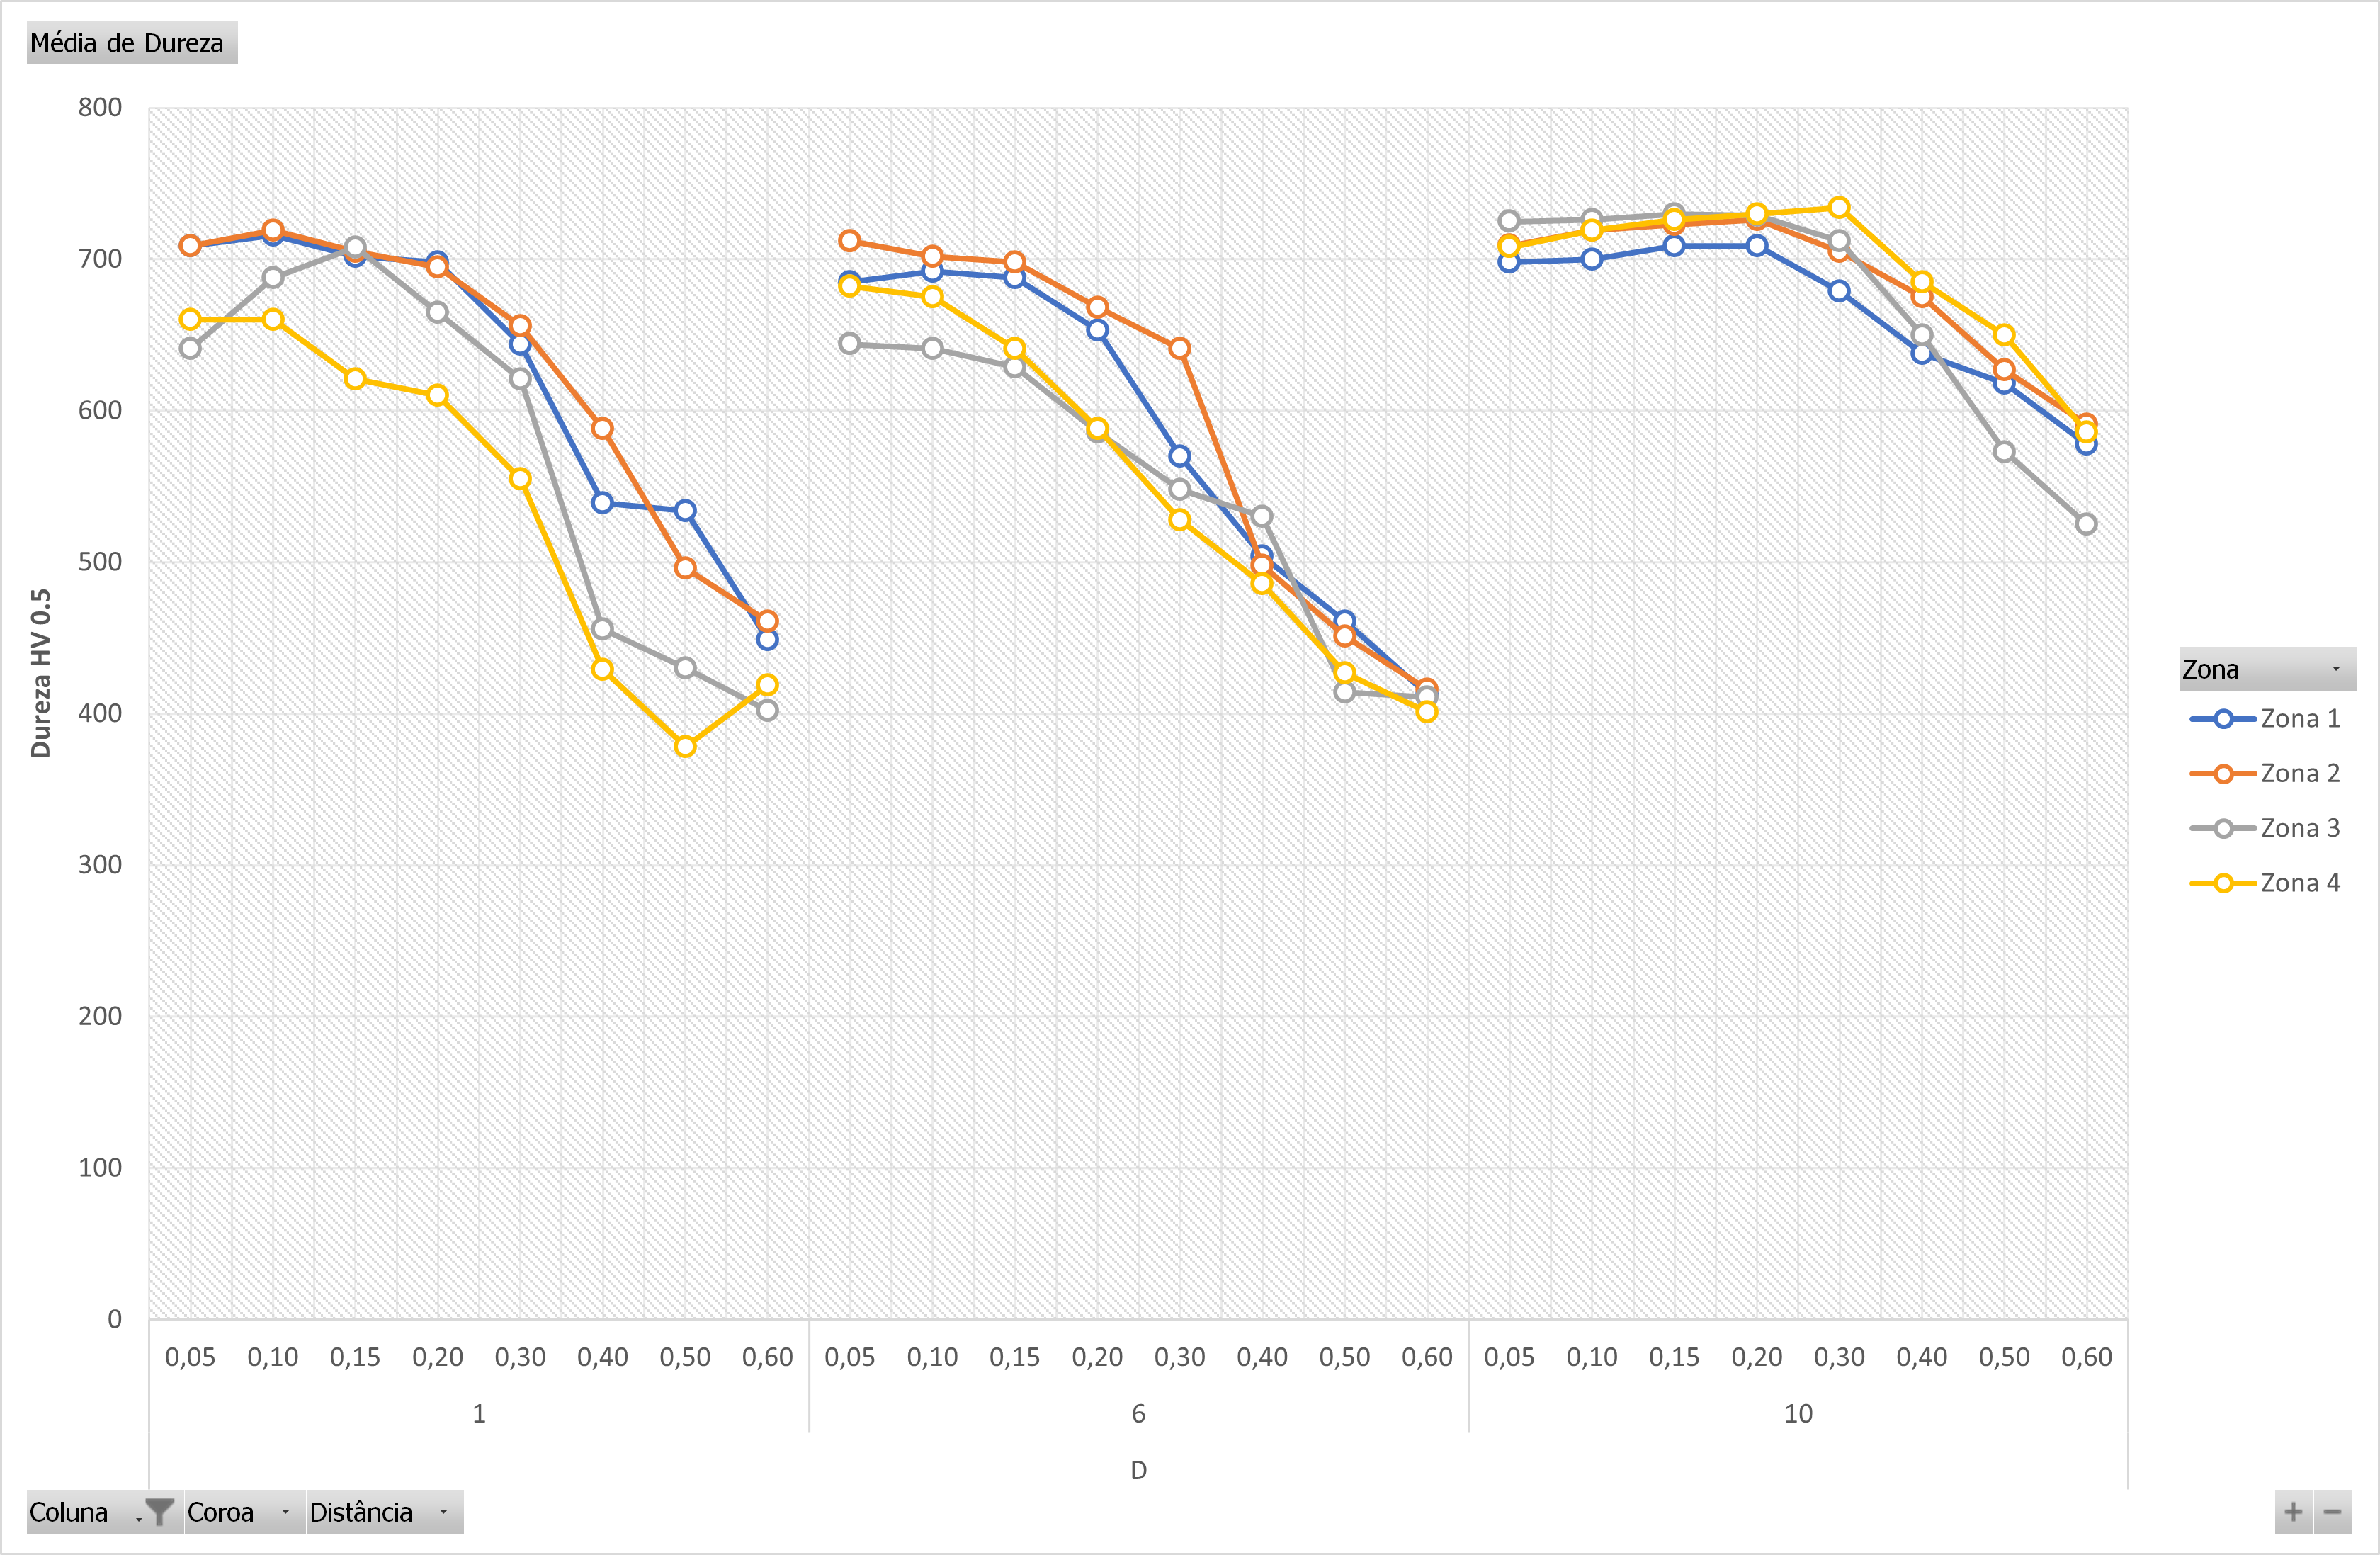
\includegraphics[width = 0.9\textwidth]{Figures/Cap4/Grafico_4_Zonas_ST.png}
        \caption{}
        \label{fig:resultados_ST}
    \end{subfigure}
    \caption[Filiações de dureza das quatro zonas na roda de coroa DB45 Nº 1]%
    {Gráficos das filiações de dureza das quatro zonas nas rodas de coroa protegidas por tampa Y, protegidas por tampa O, e protegida por tampa P, e sem tampa de proteção, respetivamente.}
\end{figure}
%%%%%%%%%%%%%%%%%%%%%%%%%%%%%%%%%%%%%%%%%%%%%%%%%%%%%%%%%%%%%%%%%%%%%%%%%%%%%
\newpage
\par
Vê-se claramente uma diminuição nos níveis de dureza em todos os tipos de ferramentas de proteção com tampa. No entanto, na ferramenta sem tampa, onde apenas é protegida a parte de baixo, não se nota uma alteração significativa nos níveis de dureza. Isso confirma duas teorias. Uma que não há impactos significativos da geometria da tampa no resultado da proteção, no entanto, o uso de uma tampa é imprescindível para o funcionamento do sistema. É importante também mencionar que não foi proposta uma solução que não utilizasse uma proteção na parte de baixo, uma vez que o fluido de têmpera é carregado de baixo para cima no tanque de têmpera, o que poderia resultar na remoção da tampa pelo fluido de têmpera, e numa possível avaria no sistema de têmpera. Novamente, vê-se nas Figuras \ref{{fig:resultados_4T_dent}} que não há alterações significativas nas durezas do dentado em nenhuma das soluções propostas.
%%%%%%%%%%%%%%%%%%%%%%%%%%%%%%%%%%%%%%%%%%%%%%%%%%%%%%%%%%%%%%%%%%%%%%%%%%%%%
\begin{figure}[htb]
    \centering
    \begin{subfigure}{.4\textwidth}\
        \centering
        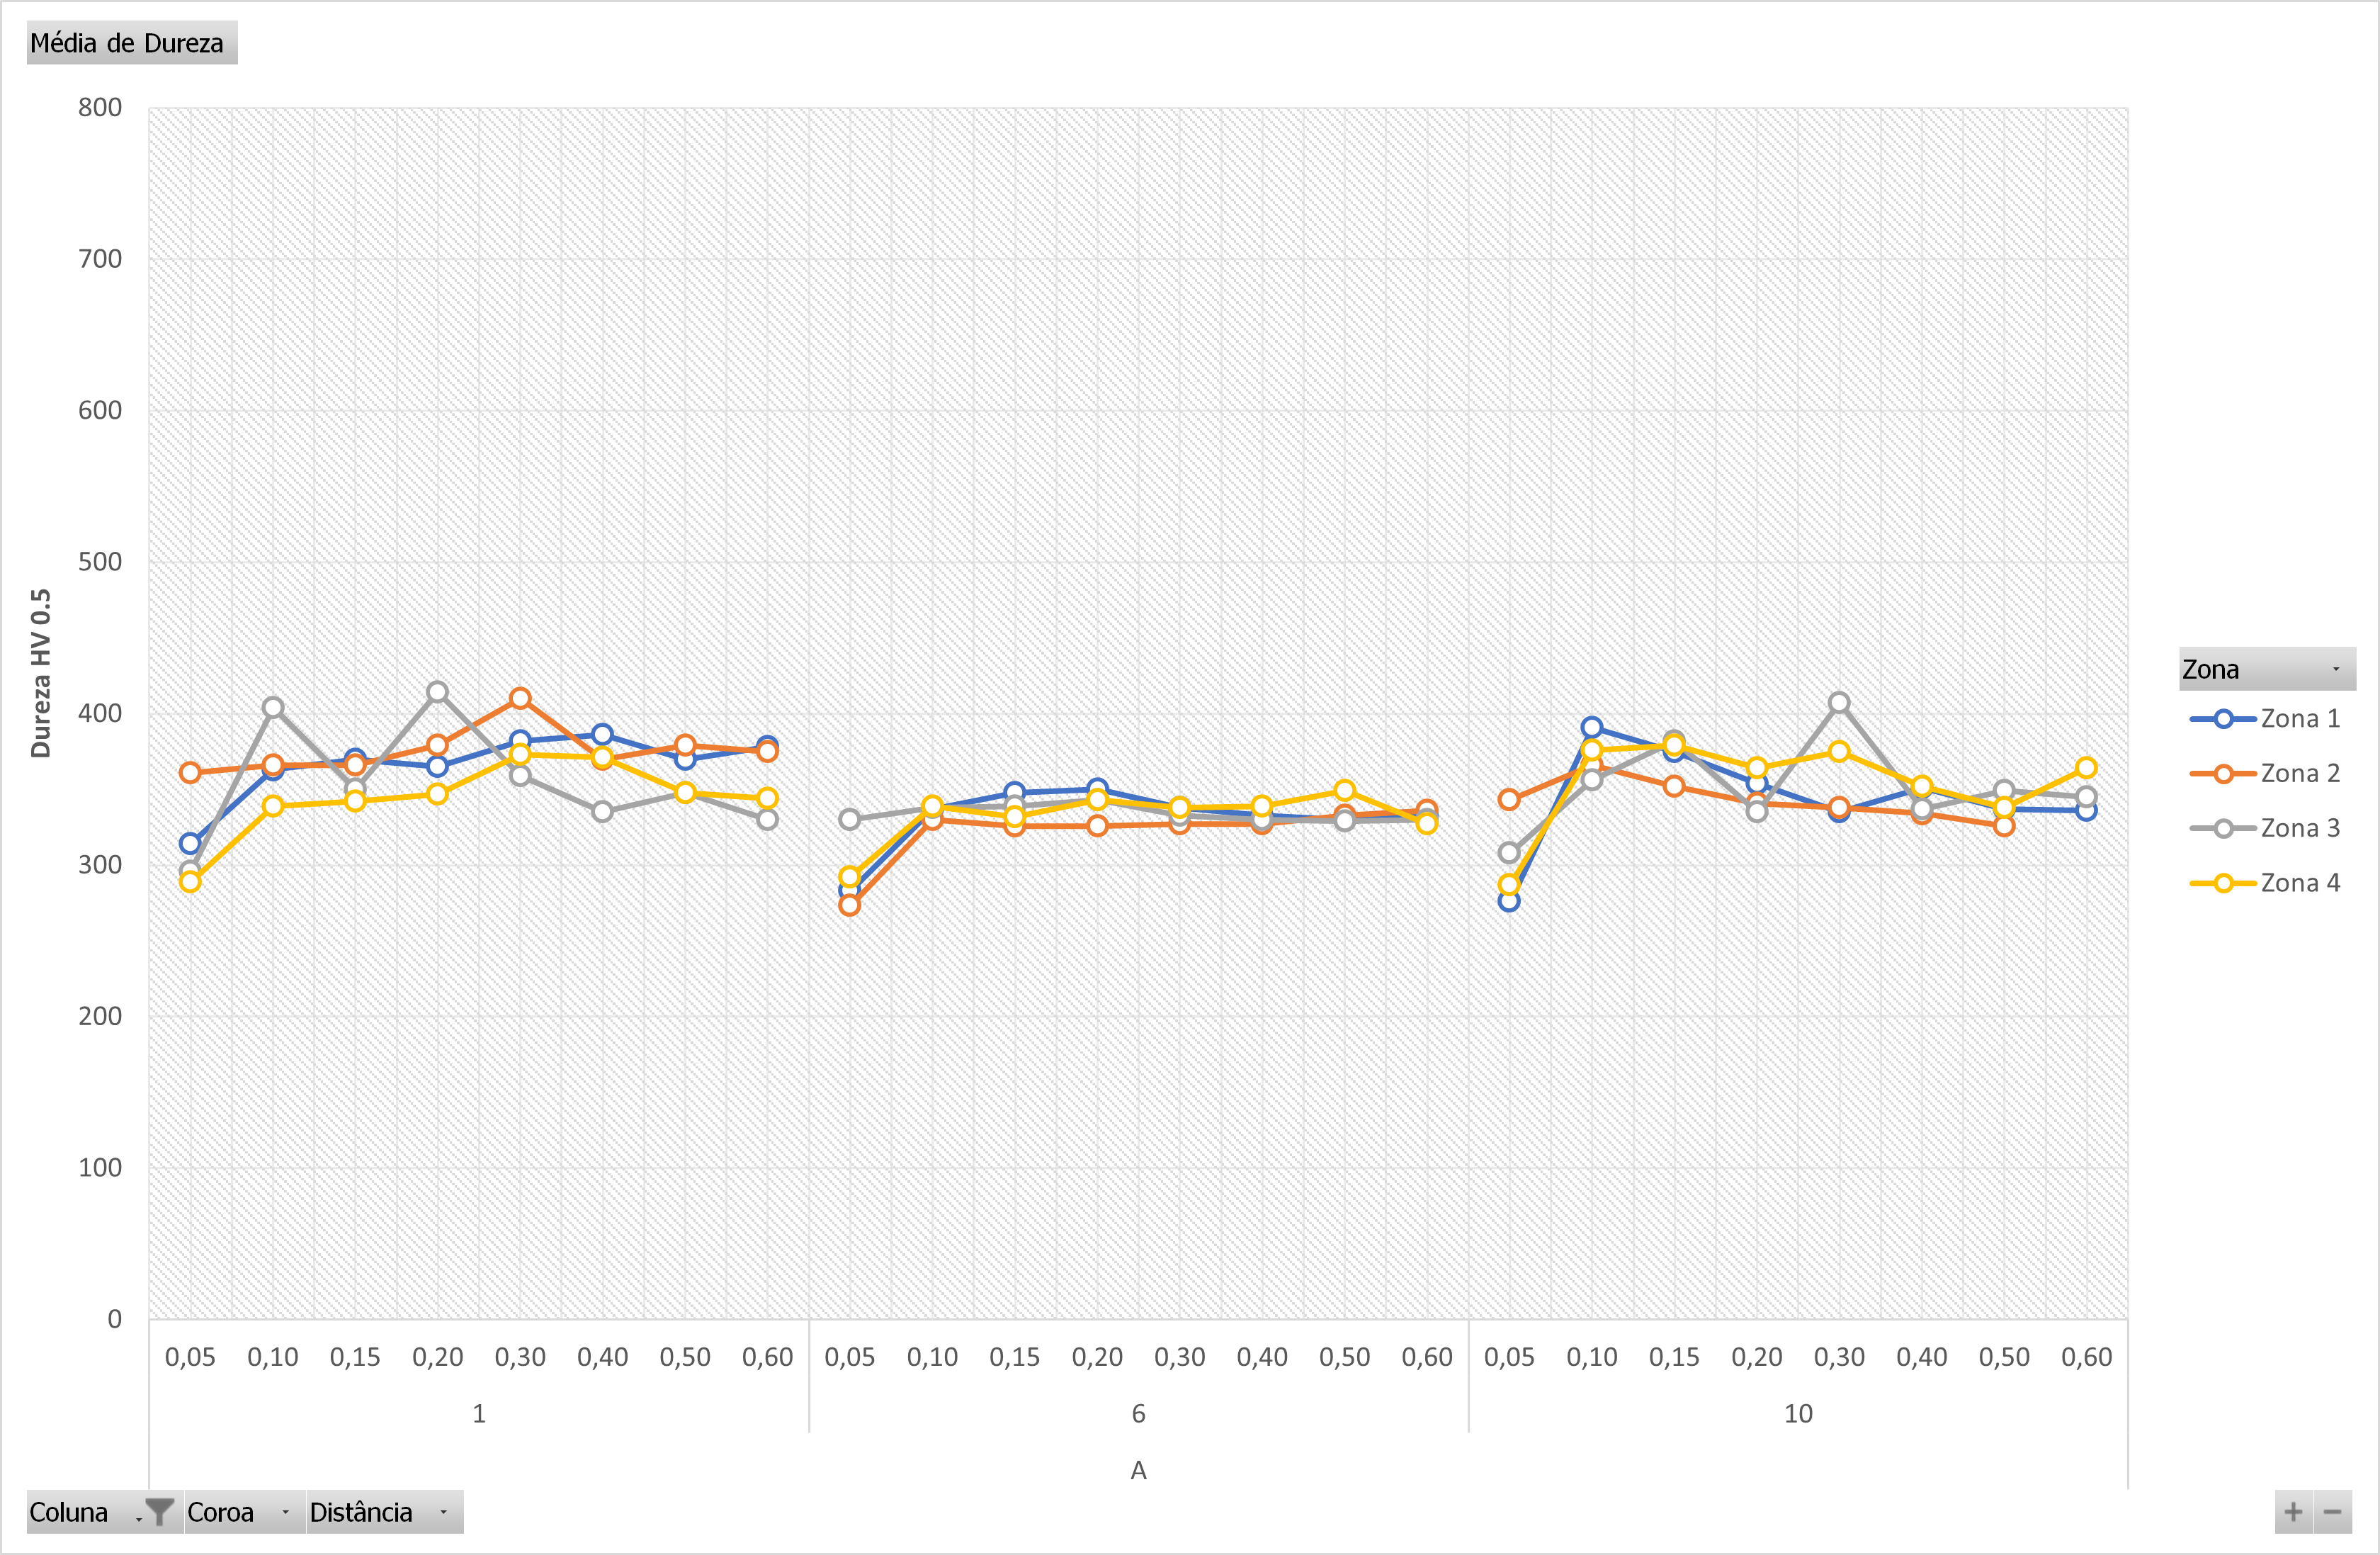
\includegraphics[width = 0.9\textwidth]{Figures/Cap4/Grafico_4_Zonas_Y.png}
        \caption{}
        \label{fig:resultados_Tampa_Y_dent}
    \end{subfigure}%
    \begin{subfigure}{.4\textwidth}
        \centering
        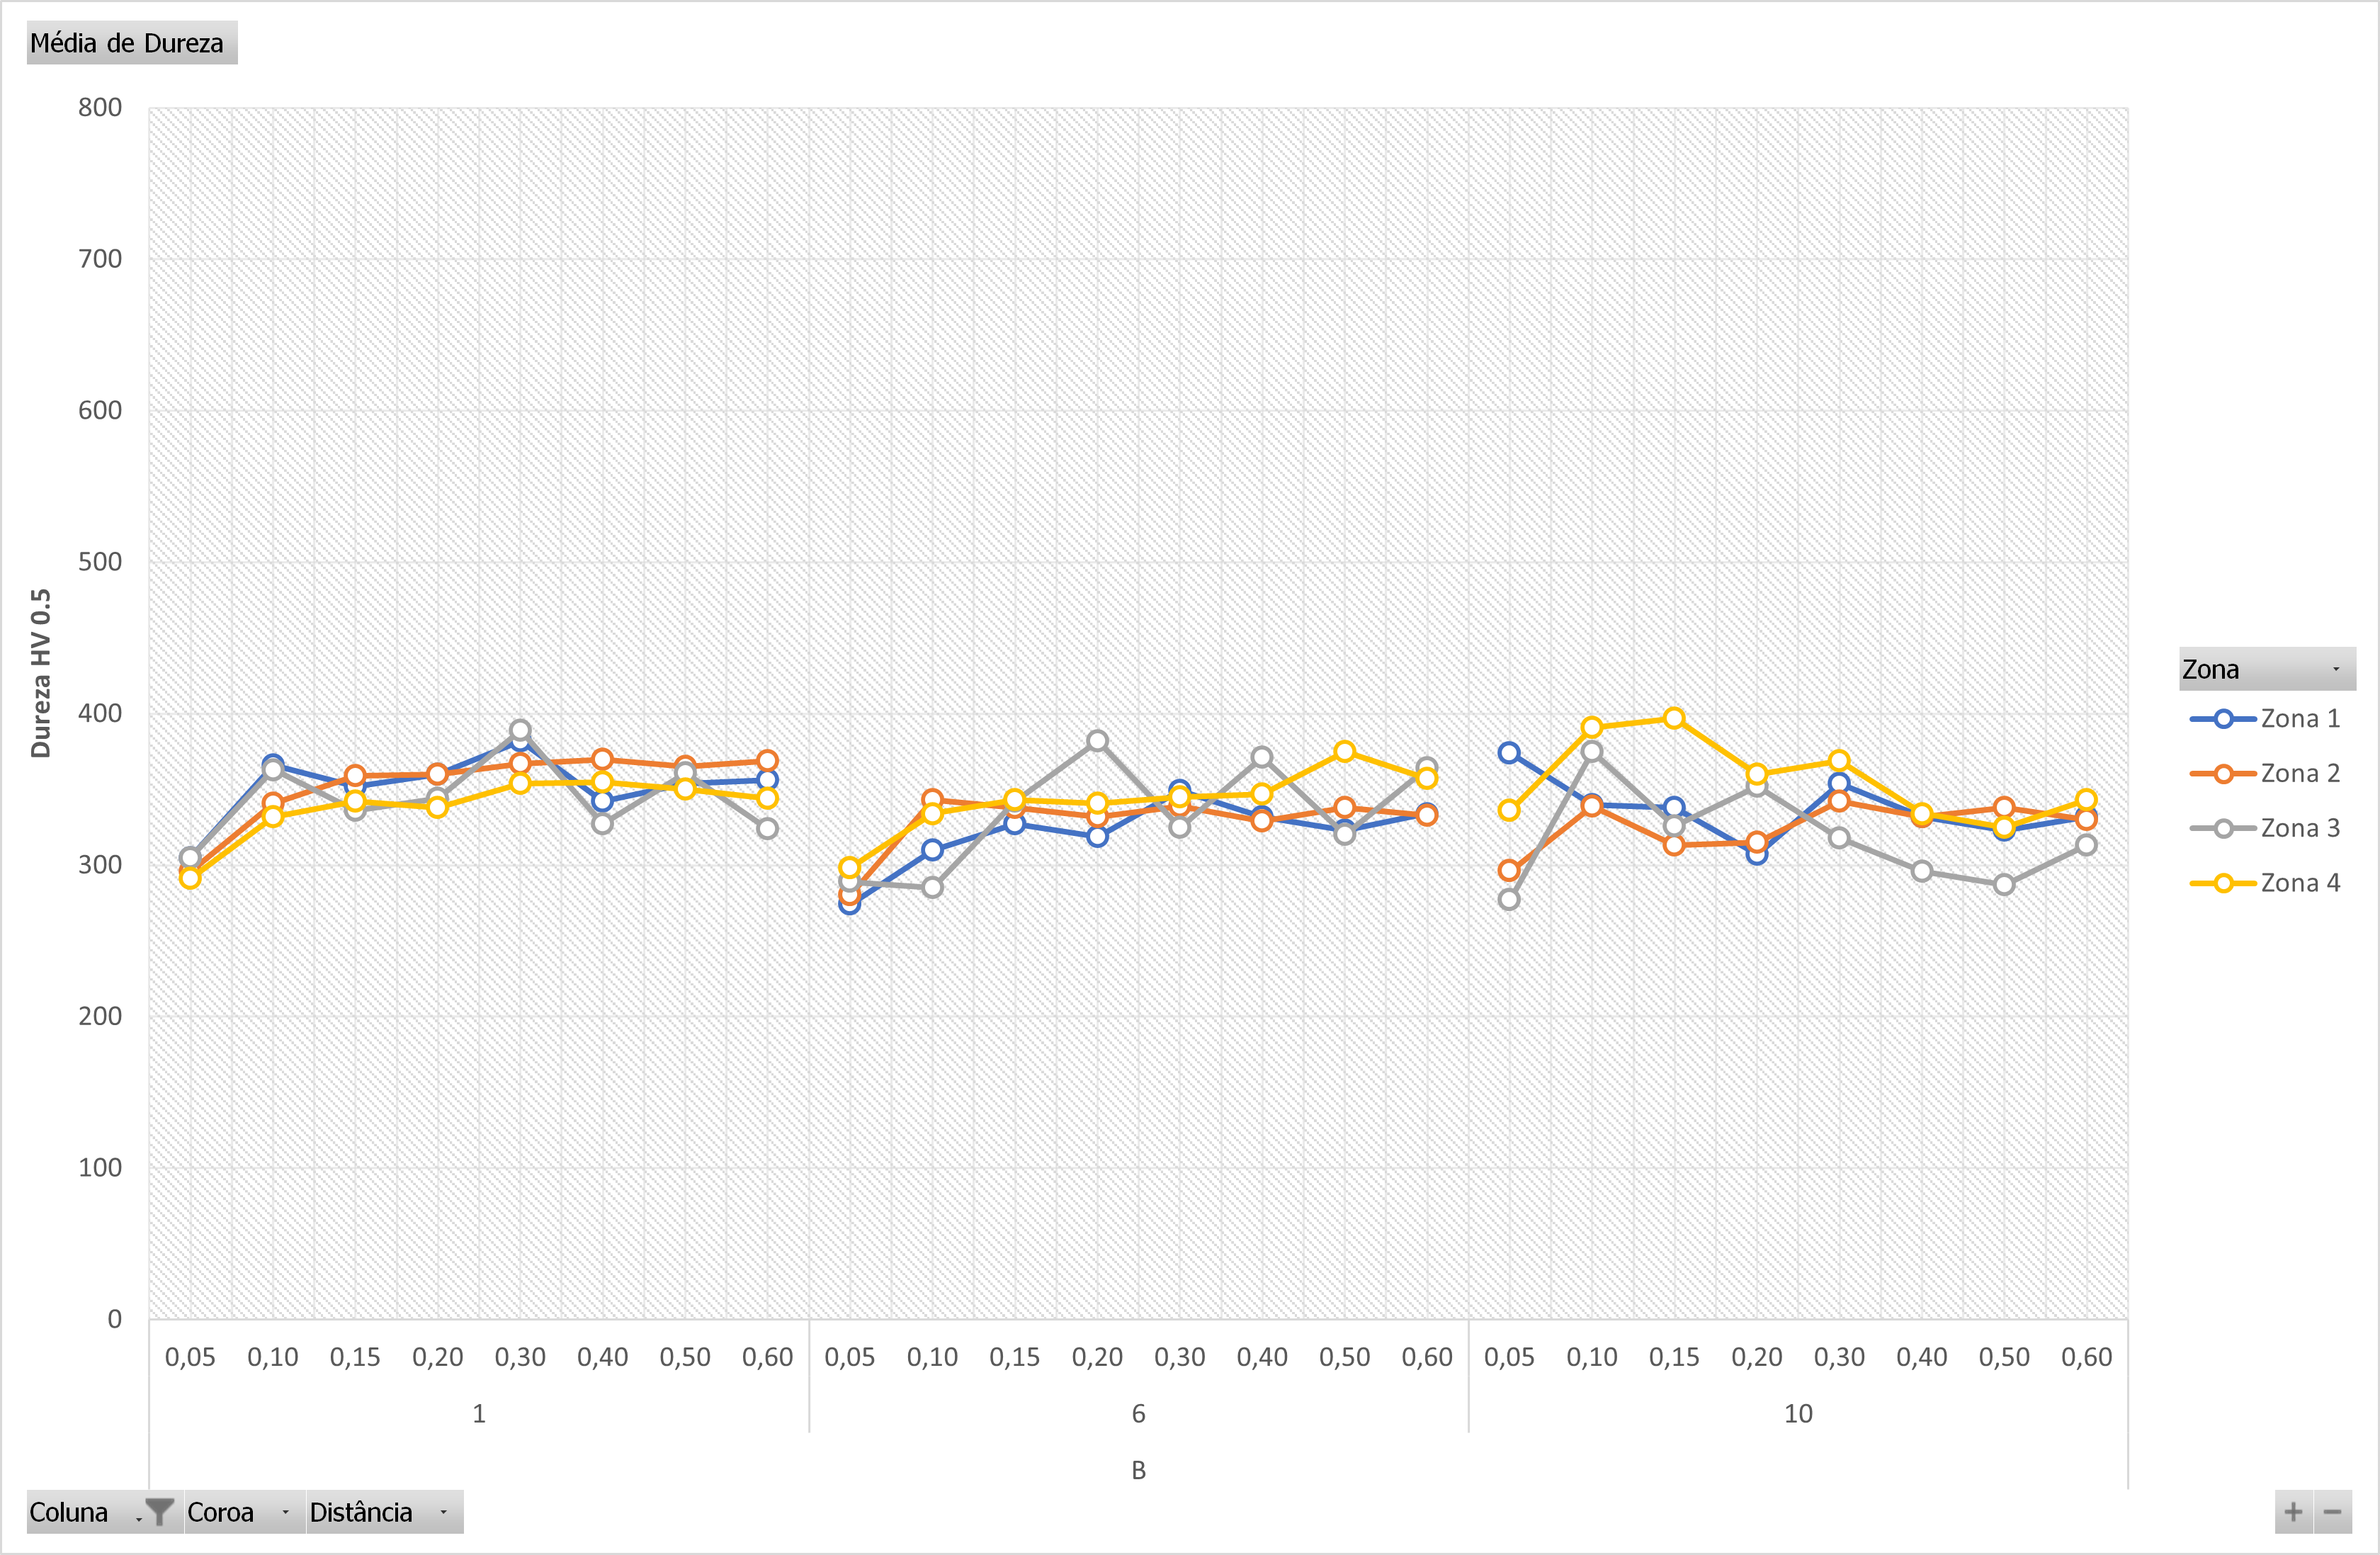
\includegraphics[width = 0.9\textwidth]{Figures/Cap4/Grafico_4_Zonas_O.png}
        \caption{}
        \label{fig:resultados_Tampa_O_dent}
    \end{subfigure}
    \begin{subfigure}{.4\textwidth}\
        \centering
        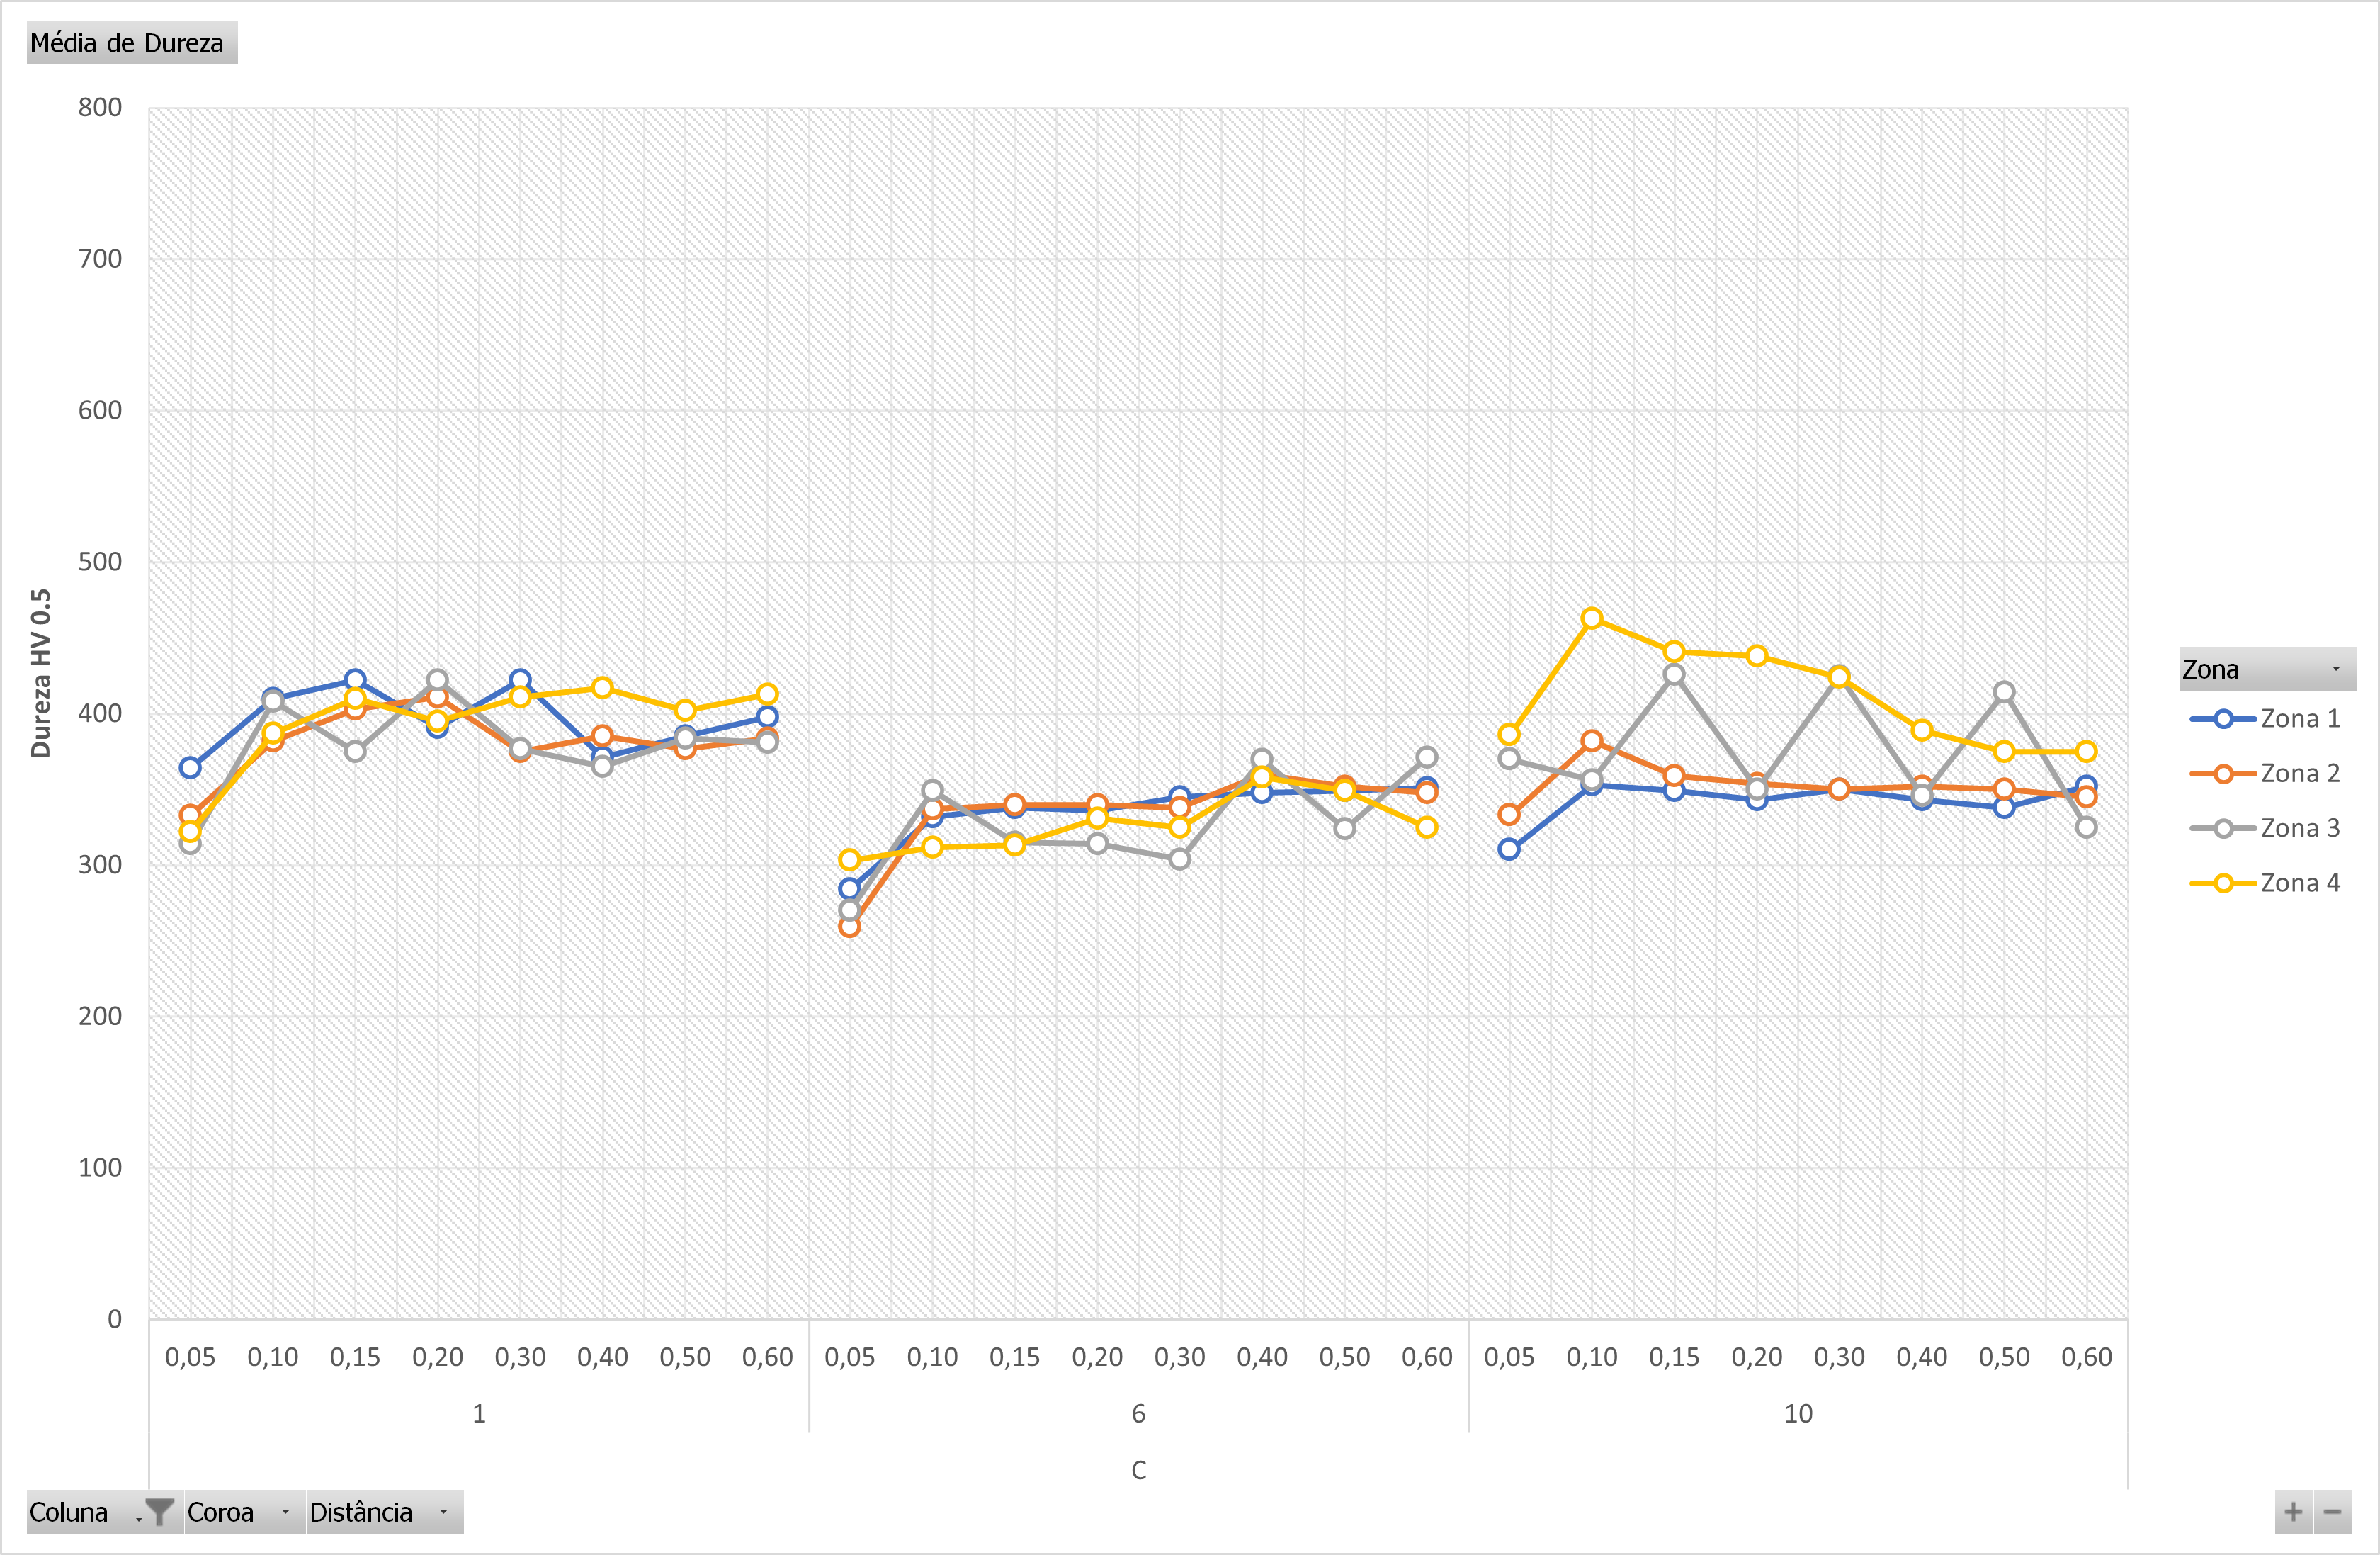
\includegraphics[width = 0.9\textwidth]{Figures/Cap4/Grafico_4_Zonas_P.png}
        \caption{}
        \label{fig:resultados_Tampa_P_dent}
    \end{subfigure}%
    \begin{subfigure}{.4\textwidth}
        \centering
        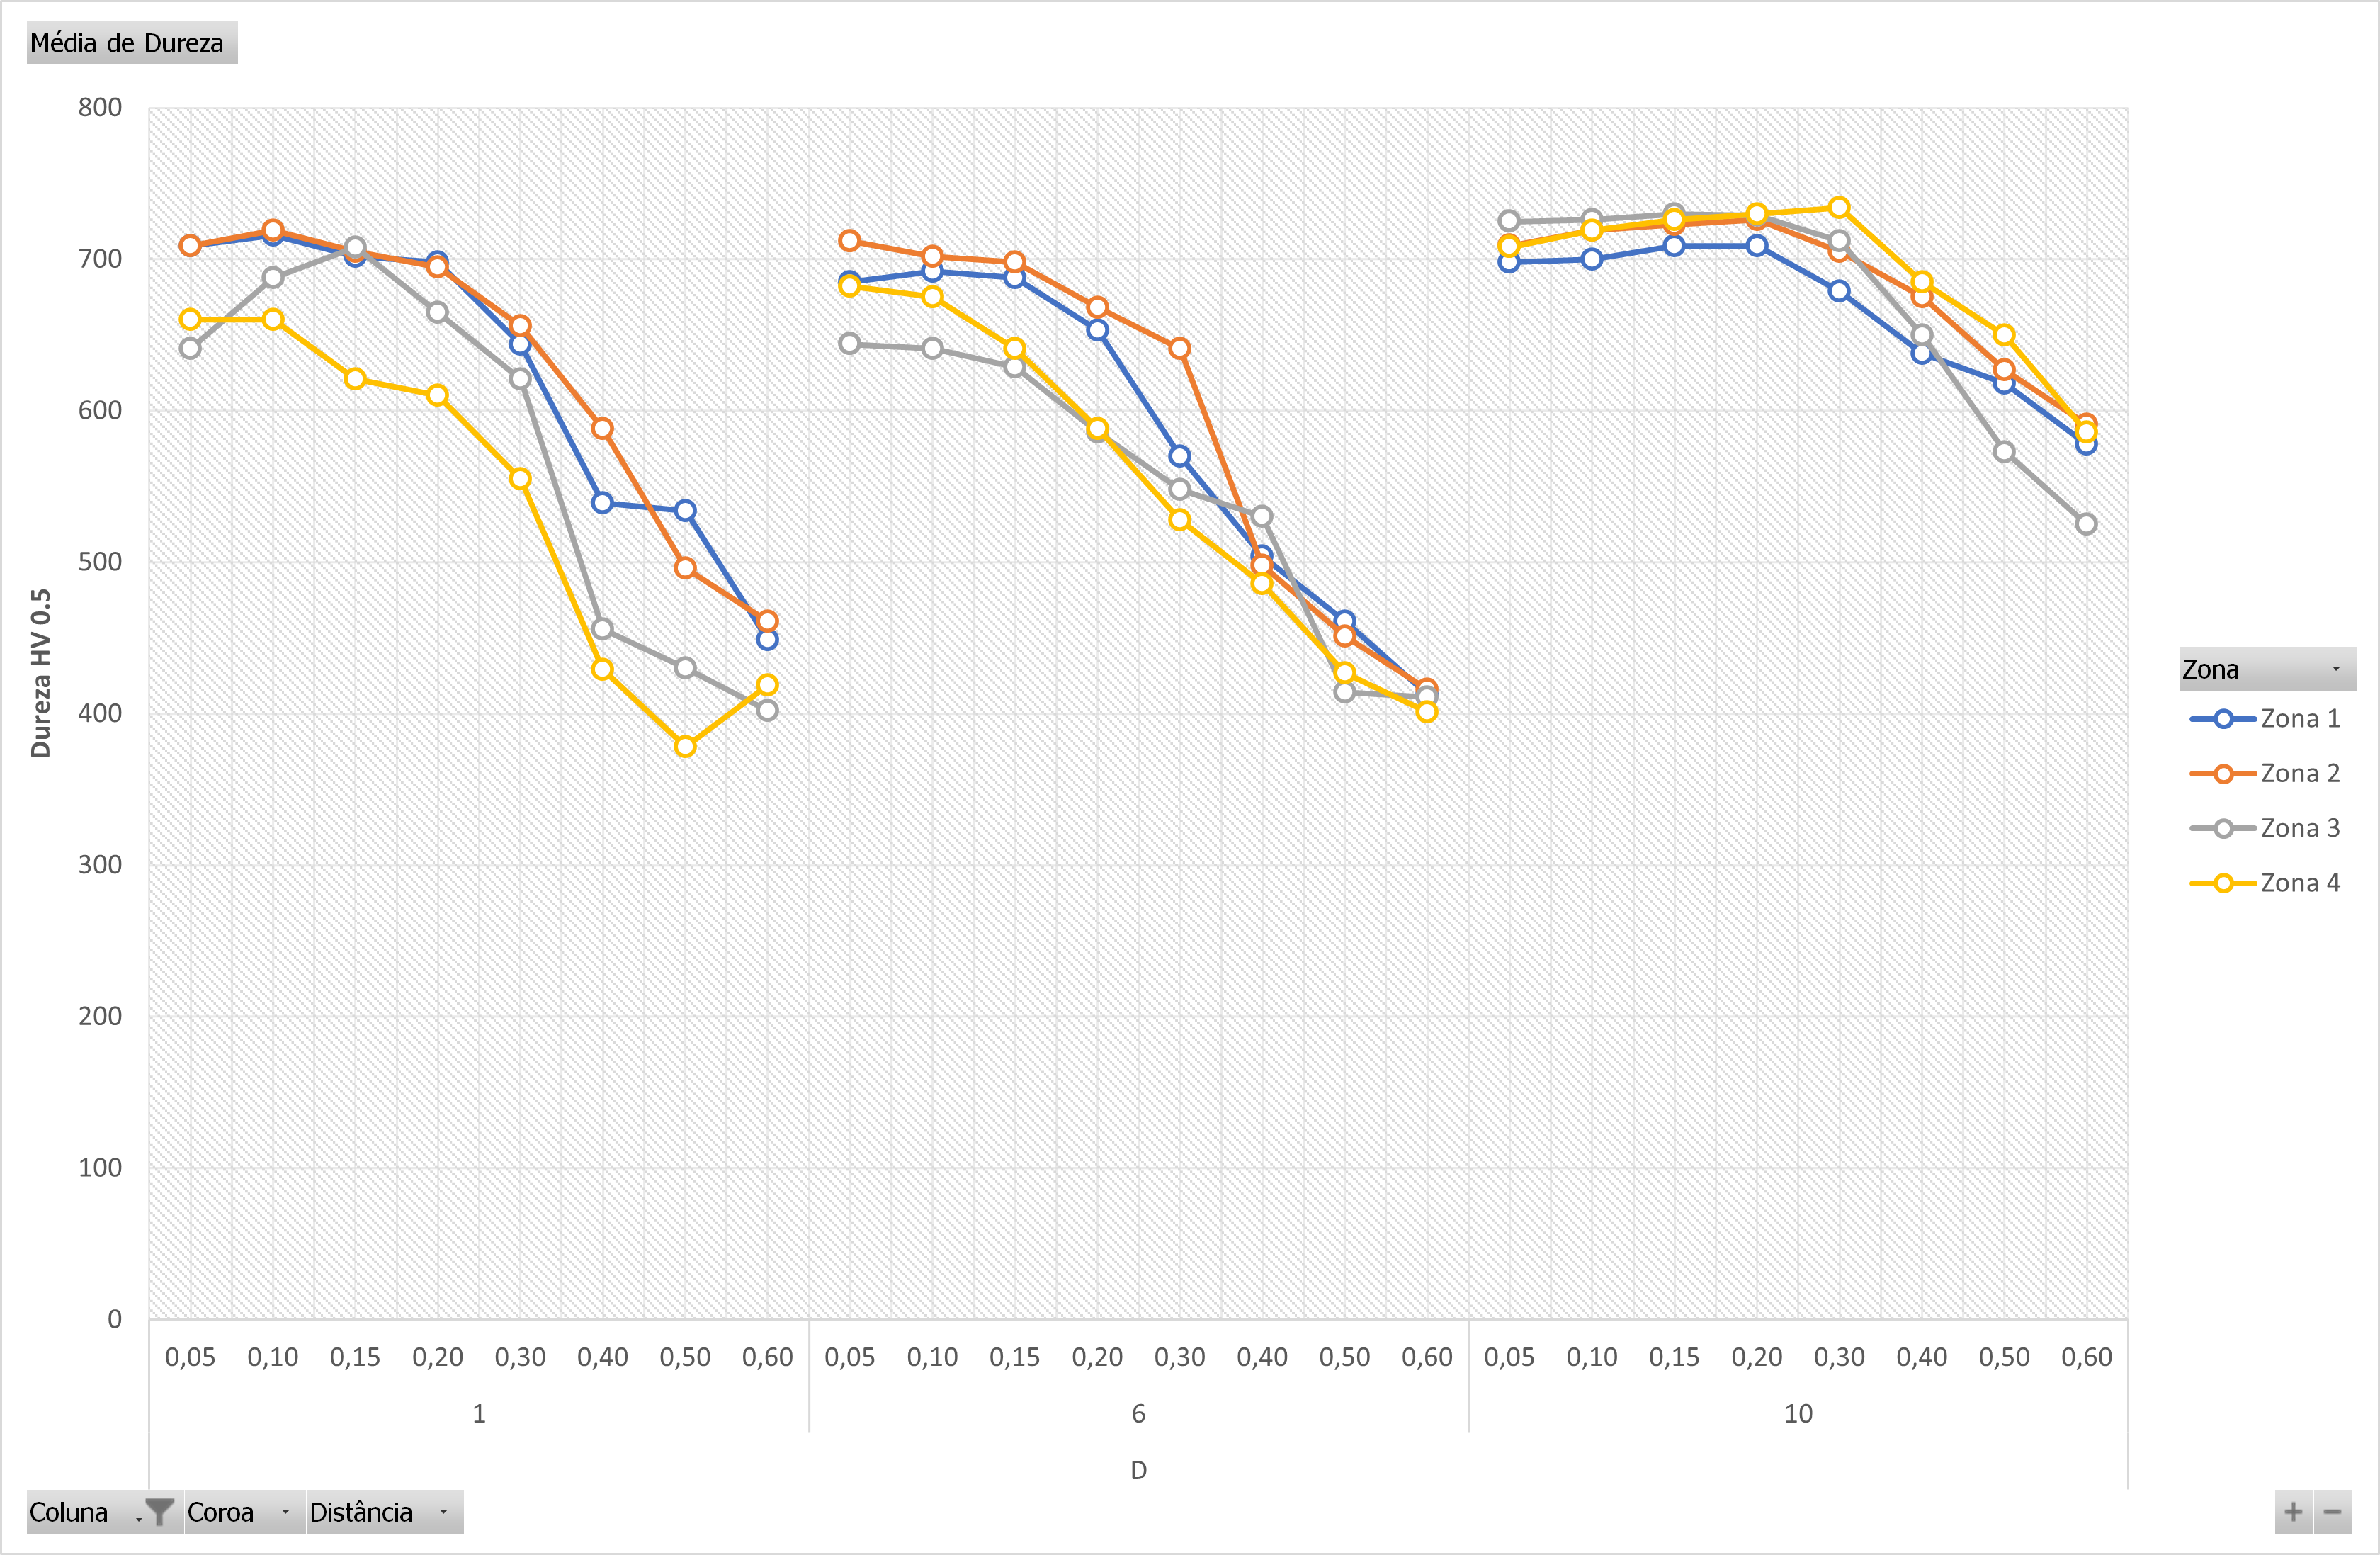
\includegraphics[width = 0.9\textwidth]{Figures/Cap4/Grafico_4_Zonas_ST.png}
        \caption{}
        \label{fig:resultados_ST_dent}
    \end{subfigure}
    \label{fig:resultados_4T_dent}
    \caption[Filiações de dureza das quatro zonas na roda de coroa DB45 Nº 1]%
    {Gráficos das filiações de dureza das quatro zonas nas rodas de coroa protegidas por tampa Y, protegidas por tampa O, e protegida por tampa P, e sem tampa de proteção, respetivamente.}
\end{figure}
%%%%%%%%%%%%%%%%%%%%%%%%%%%%%%%%%%%%%%%%%%%%%%%%%%%%%%%%%%%%%%%%%%%%%%%%%%%%%